%Version 3.1 December 2024
% See section 11 of the User Manual for version history
%
%%%%%%%%%%%%%%%%%%%%%%%%%%%%%%%%%%%%%%%%%%%%%%%%%%%%%%%%%%%%%%%%%%%%%%
%%                                                                 %%
%% Please do not use \input{...} to include other tex files.       %%
%% Submit your LaTeX manuscript as one .tex document.              %%
%%                                                                 %%
%% All additional figures and files should be attached             %%
%% separately and not embedded in the \TeX\ document itself.       %%
%%                                                                 %%
%%%%%%%%%%%%%%%%%%%%%%%%%%%%%%%%%%%%%%%%%%%%%%%%%%%%%%%%%%%%%%%%%%%%%

%%\documentclass[referee,sn-basic]{sn-jnl}% referee option is meant for double line spacing

%%=======================================================%%
%% to print line numbers in the margin use lineno option %%
%%=======================================================%%

%%\documentclass[lineno,pdflatex,sn-basic]{sn-jnl}% Basic Springer Nature Reference Style/Chemistry Reference Style

%%=========================================================================================%%
%% the documentclass is set to pdflatex as default. You can delete it if not appropriate.  %%
%%=========================================================================================%%



%%Note: the following reference styles support Namedate and Numbered referencing. By default the style follows the most common style. To switch between the options you can add or remove “Numbered” in the optional parenthesis. 
%%The option is available for: sn-basic.bst, sn-chicago.bst%  
 
%%\documentclass[pdflatex,sn-nature]{sn-jnl}% Style for submissions to Nature Portfolio journals

% Figures are supplied as EPS files.
\RequirePackage{iftex}
\ifXeTeX\PassOptionsToClass{pdflatex}{sn-jnl}\fi
\ifPDFTeX\ifnum\pdfoutput>0 \PassOptionsToClass{pdflatex}{sn-jnl}\fi\fi
\documentclass[sn-basic]{sn-jnl}% Basic Springer Nature author-year style
%%\documentclass[pdflatex,sn-mathphys-ay]{sn-jnl}% Math and Physical Sciences Author Year Reference Style
%%\documentclass[pdflatex,sn-aps]{sn-jnl}% American Physical Society (APS) Reference Style
%%\documentclass[pdflatex,sn-vancouver-num]{sn-jnl}% Vancouver Numbered Reference Style
%%\documentclass[pdflatex,sn-vancouver-ay]{sn-jnl}% Vancouver Author Year Reference Style
%%\documentclass[pdflatex,sn-apa]{sn-jnl}% APA Reference Style
%%\documentclass[pdflatex,sn-chicago]{sn-jnl}% Chicago-based Humanities Reference Style

%%%% Standard Packages
%%<additional latex packages if required can be included here>

\usepackage{graphicx}%
\usepackage{multirow}%
\usepackage{amsmath,amssymb,amsfonts}%
\usepackage{amsthm}%

\usepackage[title]{appendix}%
\usepackage{xcolor}%
\usepackage{textcomp}%

\usepackage{booktabs}%




\usepackage{array}%
\usepackage{tabularx}%
\usepackage{rotating}%
%%%%

%%%%%=============================================================================%%%%
%%%%  Remarks: This template is provided to aid authors with the preparation
%%%%  of original research articles intended for submission to journals published 
%%%%  by Springer Nature. The guidance has been prepared in partnership with 
%%%%  production teams to conform to Springer Nature technical requirements. 
%%%%  Editorial and presentation requirements differ among journal portfolios and 
%%%%  research disciplines. You may find sections in this template are irrelevant 
%%%%  to your work and are empowered to omit any such section if allowed by the 
%%%%  journal you intend to submit to. The submission guidelines and policies 
%%%%  of the journal take precedence. A detailed User Manual is available in the 
%%%%  template package for technical guidance.
%%%%%=============================================================================%%%%

%% as per the requirement new theorem styles can be included as shown below
\theoremstyle{thmstyleone}%
\newtheorem{theorem}{Theorem}%  meant for continuous numbers
%%\newtheorem{theorem}{Theorem}[section]% meant for sectionwise numbers
%% optional argument [theorem] produces theorem numbering sequence instead of independent numbers for Proposition
\newtheorem{proposition}[theorem]{Proposition}% 
%%\newtheorem{proposition}{Proposition}% to get separate numbers for theorem and proposition etc.

\theoremstyle{thmstyletwo}%
\newtheorem{example}{Example}%
\newtheorem{remark}{Remark}%

\theoremstyle{thmstylethree}%
\newtheorem{definition}{Definition}%

\geometry{textheight=243mm}
\raggedbottom
%%\unnumbered% uncomment this for unnumbered level heads

\begin{document}

\title[Identifying hosts affected by omissions in an agentic external reconnaissance pipeline]{Identifying hosts affected by omissions in an agentic external reconnaissance pipeline: a fault injection study}
%%=============================================================%%
%% GivenName	-> \fnm{Joergen W.}
%% Particle	-> \spfx{van der} -> surname prefix
%% FamilyName	-> \sur{Ploeg}
%% Suffix	-> \sfx{IV}
%% \author*[1,2]{\fnm{Joergen W.} \spfx{van der} \sur{Ploeg} 
%%  \sfx{IV}}\email{iauthor@gmail.com}
%%=============================================================%%

\author[1]{\fnm{Xuan} \sur{Chen}}\email{3079284258@qq.com}
\author[1]{\fnm{Kai} \sur{Yi}}\email{1437132005@qq.com}
\author[1]{\fnm{Haodong} \sur{Wang}}\email{15870627237@163.com}
\author*[1]{\fnm{Xiangmin} \sur{Ji}}\email{jixm168@126.com}

\affil*[1]{\orgname{Fujian Agriculture and Forestry University},
  \orgaddress{\city{Fuzhou}, \postcode{350002}, \state{Fujian}, \country{China}}}

\abstract{An external reconnaissance pipeline may omit a discovered host from the handoff to evidence collection or drop evidence for that host during downstream processing. We studied these mechanisms using nine fault variants across 20 purposively selected organizations, yielding 180 faulted runs and 260 injected run--host pairs. For each of four variants, all 20 clean--faulted pairs had identical prediction sets and F1 scores (the harmonic mean of precision and recall) on all four asset measures, despite differences in the evidence records. Surviving evidence named the target host in 129 of 260 pairs. Adding the resolved-host manifest from the same faulted run raised coverage to 243 of 260. Across the 180 main-grid runs, the tie-aware top-1 hit rate was 0.735 for the rule-based localizer (Combined) and 0.456 for Isolation Forest (IF). The candidate set included every host needed for a sufficient plan in 168 of the 180 runs. When plans specified all four evidence families for each alerted host, IF covered every required action in all 168 runs and Combined did so in 145. At 43 additional injection locations in the same corpus, Domain Name System (DNS) records were the target host's only clean-run evidence. Of these locations, 42 had an affected, leaf-repairable output, and the target was absent from the candidate set in all 42. In this pipeline, candidate visibility limited which hosts could be addressed. Combined more often ranked a target first, while IF alerts yielded more sufficient offline plans.}

%%================================%%
%% Sample for structured abstract %%
%%================================%%

% \abstract{\textbf{Purpose:} The abstract serves both as a general introduction to the topic and as a brief, non-technical summary of the main results and their implications. The abstract must not include subheadings (unless expressly permitted in the journal's Instructions to Authors), equations or citations. As a guide the abstract should not exceed 200 words. Most journals do not set a hard limit however authors are advised to check the author instructions for the journal they are submitting to.
% 
% \textbf{Methods:} The abstract serves both as a general introduction to the topic and as a brief, non-technical summary of the main results and their implications. The abstract must not include subheadings (unless expressly permitted in the journal's Instructions to Authors), equations or citations. As a guide the abstract should not exceed 200 words. Most journals do not set a hard limit however authors are advised to check the author instructions for the journal they are submitting to.
% 
% \textbf{Results:} The abstract serves both as a general introduction to the topic and as a brief, non-technical summary of the main results and their implications. The abstract must not include subheadings (unless expressly permitted in the journal's Instructions to Authors), equations or citations. As a guide the abstract should not exceed 200 words. Most journals do not set a hard limit however authors are advised to check the author instructions for the journal they are submitting to.
% 
% \textbf{Conclusion:} The abstract serves both as a general introduction to the topic and as a brief, non-technical summary of the main results and their implications. The abstract must not include subheadings (unless expressly permitted in the journal's Instructions to Authors), equations or citations. As a guide the abstract should not exceed 200 words. Most journals do not set a hard limit however authors are advised to check the author instructions for the journal they are submitting to.}

\keywords{software reliability, evidence pipelines, candidate visibility, fault localization, offline action planning}

%%\pacs[JEL Classification]{D8, H51}

%%\pacs[MSC Classification]{35A01, 65L10, 65L12, 65L20, 65L70}

\maketitle

\section{Introduction}\label{sec:introduction}

A structured evidence pipeline can fail without reporting an explicit error when it omits a discovered and resolved host from the output passed to evidence collection or excludes an existing evidence record from a downstream processing view. Even when the pipeline completes, the retained diagnostic state may contain no signal identifying the omission and the host or record involved. In this pipeline, a localizer can rank an affected host only if the candidate set includes its identity. Following \citet{avizienis2004}, we use fault for the injected change, error for the resulting incorrect pipeline state, and failure for an observable deviation from the expected pipeline output.

We use host identities to track which of the four diagnostic stages each host reaches: candidate generation $\rightarrow$ ranking $\rightarrow$ alerting $\rightarrow$ action planning.

The localizer ranks the hosts selected during candidate generation and flags those that meet its alert criterion. The planner then specifies which evidence families to reacquire for each flagged host. If the records used to generate a run's candidate set do not identify a host, the localizer cannot score that host in that run.

We study an external reconnaissance pipeline that combines software tools with processing assisted by large language models (LLMs). Its five stages are discovery, evidence collection, fusion, decision, and reporting. The pipeline stores Domain Name System (DNS), certificate, Hypertext Transfer Protocol (HTTP), registration, and third-party network observations as structured evidence. A directed acyclic graph (DAG) links this evidence to derived claims, decisions, and report items. LLMs assist selected upstream stages, while the diagnostic methods use only the stored structured records and do not require LLM reasoning traces. We use “agentic” to describe the pipeline architecture; this study does not evaluate multi-agent coordination or trajectory-based diagnosis.

We call an omission provenance-silent when the retained diagnostic state contains no signal that both identifies the omission and names the affected record or host. This definition covers the five persisted record streams in Section~\ref{sec:pipeline-evidence-dag} and the derived validator output. A record may name a host, and the validator may flag it for revalidation, without identifying which evidence is missing. We measured host visibility and validator coverage. The archived records did not provide enough information to estimate how common provenance-silent omissions were.

Software fault-localization methods rank program elements using execution data \citep{wong2016flsurvey}. In agent systems, related methods use recorded trajectories to score actions or identify the agent and step responsible for a failure \citep{famas,whowhen2025}. Why-not provenance and negative provenance explain why a specified, expected result or event is missing \citep{chapman2009whynot,herschel2010spjua,wu2014negativeprovenance}. Our question is whether faulted-run records preserve the host identity needed to define a candidate before ranking begins. This distinction informs instrumentation and persistence decisions in software pipelines.

We replayed the pipeline with omissions injected at two boundaries. F4 excludes evidence from the decision-stage normalized view, whereas F10 removes a discovered and resolved host from the asset mapping passed downstream after discovery returns. Across 20 purposively selected organizations, six F4 and three F10 variants produced 180 faulted experimental units and 260 injected run--host pairs. We selected injection targets from each organization's clean bundle. When processing a faulted run, the localizers and planner had no access to its paired clean bundle or injection labels. We used the recorded targets to evaluate localization and the paired records to derive the required reacquisition actions. We calibrated the statistical baselines' alert thresholds using clean runs from the other 19 organizations.

We address three research questions:
\begin{enumerate}
    \item \textbf{RQ1 (Failure effects and validator coverage).} Which omission variants change the four measured asset-level F1 scores, and how often does the retained validator signal flag an injected host?
    \item \textbf{RQ2 (Candidate visibility and localization).} In how many injected run--host pairs does the target host enter the candidate set? How accurately do the localizers rank and flag targets under this rule?
    \item \textbf{RQ3 (Offline planning).} How do detector alerts and family-selection policies affect offline plan sufficiency and weighted plan cost under a four-family action contract?
\end{enumerate}

Across all nine variants, surviving evidence named the injected host in 129 of 260 run--host pairs. Adding the same-run resolved-host manifest brought the target host into the candidate set for 114 additional pairs, raising coverage to 243 of 260. In the additional DNS-only sample, all 42 consequence-eligible targets lacked the IP-bearing entry required for manifest inclusion. In the main grid, adding surviving claim subjects to the candidate set raised coverage to 254 of 260 pairs.

The tie-aware Detect@1 hit rates were 0.735 for Combined and 0.456 for Isolation Forest (IF). At the operating points used in the main analysis, IF flagged 243 of the 260 target run--host pairs and Combined flagged 221.

Across runs, 404 of the 427 required host--family instances involved hosts in the candidate set for that run. Combined flagged hosts accounting for 380 instances, and its selective plans covered 352. Fixed-four plans specified more actions and covered requirements missed by selective plans.

\section{Related Work}\label{sec:related-work}

\subsection{Missing Results, Missing Events, and Candidate Observation Contracts}\label{sec:missing-results}

Database provenance and lineage relate query results to source records \citep{buneman2001,cui2000}. Provenance semirings formalize these relationships \citep{green2007}, and surveys compare approaches to representing them \citep{cheney2009,herschel2017}. In our study, a candidate observation contract defines which retained records can supply host identities to the localizer (Section~\ref{sec:candidate-visibility}).

The why-not approach starts with an expected but missing query result and identifies operations that may explain its absence \citep{chapman2009whynot}. In Artemis, users specify a missing answer with tuple patterns containing concrete and unknown values. The system then derives explanations from the source data \citep{herschel2010spjua}. Negative provenance similarly starts from a specified missing event and identifies conditions under which it could have occurred \citep{wu2014negativeprovenance}.

\href{https://arxiv.org/abs/2607.22448v3}{Rajan et~al. (2026)} trace information omissions to individual layers of an LLM agent pipeline. \citet{pathak2026silent} study how to detect silent failures in multi-agent trajectories, including behavioral drift and reasoning loops. In our setting, the affected host may be absent from the candidate set even when the rest of the pipeline produces an ordinary-looking output.

Software diagnosis also depends on what a system records. Console-log mining detects anomalies in production systems \citep{xu2009}, and DeepLog analyzes sequences of log events \citep{deeplog2017}. \citet{he2022} review how such records support reliability diagnosis. X-Trace links activities across layers and administrative boundaries \citep{xtrace2007}. The Dapper study describes how instrumentation and sampling affect which traces are retained \citep{sigelman2010dapper}. Pivot Tracing uses dynamic instrumentation to query activity across components \citep{mace2018pivot}. These studies show how instrumentation choices determine which identifiers are available for diagnosis.

\subsection{Software and Agent Failure Localization}\label{sec:failure-localization}

Traditional software fault localization commonly scores a predefined set of program elements using tests and coverage spectra \citep{wong2016flsurvey}. Evaluations of Tarantula and related methods measure ranking accuracy within that set \citep{abreu2007,jones2005}. \citet{parnin2011} studied how programmers use ranked results during debugging. \citet{kochhar2016} surveyed practitioners about what they expect from fault-localization tools. In our study, the elements ranked are canonical host identifiers. We vary which records can supply these identifiers and measure how that choice affects membership in the candidate set.

In agent systems, the Who\&When dataset links failures to the responsible agents and decisive error steps \citep{whowhen2025}. FAMAS uses replayed trajectories to score the suspiciousness of individual agent actions \citep{famas}, and AgentDiagnose supports visual inspection of trajectories \citep{agentdiagnose2025}. AgentRx generates constraints and checks them at each step of a trajectory. It records violations and supporting evidence, which a language model uses to identify the critical failure step \citep{agentrxreal}.

AgentDebug examines the use of corrective feedback (\href{https://arxiv.org/abs/2509.25370v1}{Zhu et~al.~2025}). Causal Agent Replay studies interventions on recorded execution steps (\href{https://arxiv.org/abs/2606.08275v1}{Shah~2026}). BLADE attributes failures by examining how receiving agents use information at source--decision handoffs (\href{https://arxiv.org/abs/2610.18780v1}{Guo et~al.~2026}).

\subsection{Empirical Failure Studies}\label{sec:empirical-failure-studies}

MAST classifies failures in multi-agent traces \citep{mast2025}. AgentChaosBench uses execution telemetry to evaluate faults injected at tool, model, guardrail, and agent boundaries \citep{zhang2026agentchaosbench}. \citet{yuan2014} traced failures in production distributed systems. \citet{natella2016} surveyed software fault-injection techniques, and \citet{alvaro2015} used data lineage to guide the selection of faults to inject. We use controlled omissions and paired comparisons to measure whether the retained records preserve the host identifier needed for candidate generation.

Our choice of experimental units and paired comparisons draws on guidance for software-engineering experiments \citep{kitchenham2002,wohlin2012}. In describing the study setting and its limits, we also draw on guidance for reporting case studies \citep{runeson2009casestudy}.

\subsection{Counterfactual Repair and Action Planning}\label{sec:counterfactual-repair}

Model-based diagnosis relates observations to a system description \citep{reiter1987}. Delta debugging uses tests to isolate the parts of an input that induce a failure \citep{zeller2002}. \href{https://arxiv.org/abs/2608.29228v2}{Li et~al. (2026)} formulate the Minimal Repair Family Recovery (MRFR) problem and propose Graph-Constrained Joint Replay (GCJR) to solve it. GCJR tests candidate event sets by counterfactual replay. We evaluate saved plans against the evidence-reacquisition actions required for each host.

The Learn--Diagnose--Plan framework uses diagnostic results to select additional tests intended to improve subsequent diagnostic accuracy \citep{elmishali2018ldp}. Our plans specify evidence reacquisition for pairs of host identifiers and evidence families. We evaluate their offline sufficiency and relative specification cost.

Automated program repair evaluates the correctness of code patches \citep{aprcacm2019}. We evaluate planned evidence-reacquisition actions using a frozen offline evaluator.

These methods explain missing results, rank recorded steps, or test interventions on graphs. We vary which faulted-run layers can name an omitted host and evaluate candidate admission, ranking, alerting, and action scope. Injection labels identify the target hosts. The evaluator derives required host--family actions from paired clean and faulted records.

\section{System Context and Fault Model}\label{sec:system-context}

\subsection{Pipeline and Evidence DAG}\label{sec:pipeline-evidence-dag}

Figure~\ref{fig:pipeline} shows the five pipeline stages and the two injection points, at the discovery handoff and in the decision-stage evidence view. The system supports dynamic routing between agents. The experiments reported here used its default static orchestration mode. Discovery identifies candidate hosts and emits a snapshot of resolved hostnames for each run. The frozen implementation builds the manifest from asset entries with an IP address. We used the final snapshot persisted for that run. Evidence collection gathers DNS records, certificate data, HTTP and favicon observations, Registration Data Access Protocol (RDAP) data, autonomous system number information, and Shodan InternetDB responses. Fusion derives claims from the collected evidence. The decision stage constructs a normalized evidence view and applies support, freshness, and policy checks before reporting produces structured results and narrative text.

The nodes of the evidence DAG are records from five persisted streams: \texttt{source\_artifact}, \texttt{evidence\_event}, \texttt{claim}, \texttt{decision}, and \texttt{report\_item}. Derivation references form its edges. Section~\ref{sec:structural-difference} defines how we match records across paired runs.

The component named \texttt{nmap} queries Shodan InternetDB for a resolved IP address without actively scanning target ports. Its \texttt{vulnerability\_applicability} claims contain Common Vulnerabilities and Exposures (CVE) identifiers returned by InternetDB. The pipeline does not independently verify these vulnerabilities. Selected upstream normalization, attribution, conflict-resolution, and reporting operations use LLMs. The localizers and planner use the persisted records. \citet{baltes2027} discuss reporting model and prompt details in LLM-based software-engineering studies. Our archive preserves only some of these details, limiting reproduction of the upstream LLM stages.

\begin{figure}[htbp]
\centering
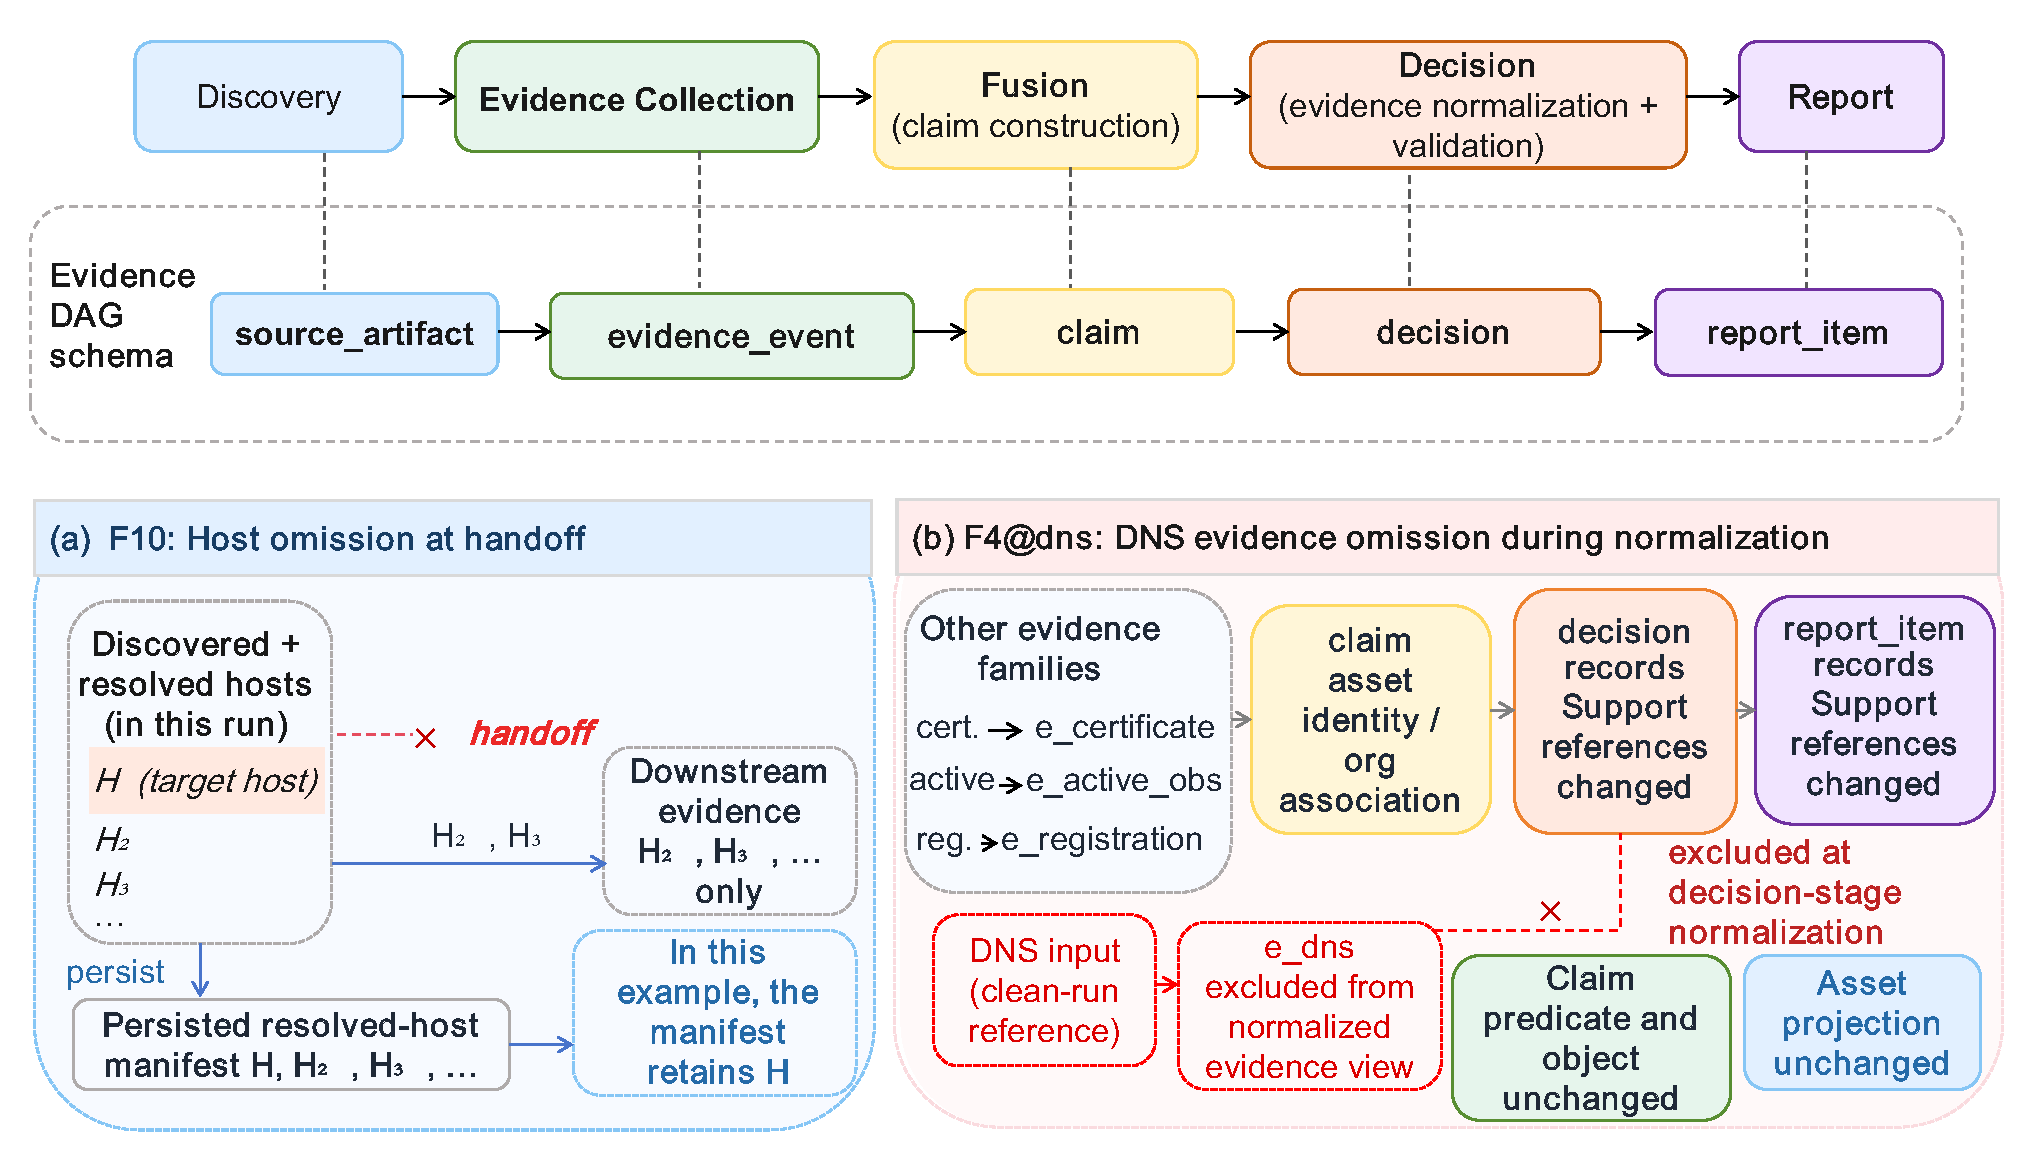
\includegraphics[width=\textwidth]{fig1}
\caption{Pipeline stages, evidence record types, and F4/F10 omission cases. F10 marks a selected host removed from the downstream asset mapping after discovery returns; surviving evidence may still name that host. F4@dns marks DNS evidence excluded from the decision-stage normalized view. In the F4@dns example, other evidence families remain available. We select targets from the clean bundle before injection and compare the paired outputs after replay}
\label{fig:pipeline}
\end{figure}

\subsection{Primary Omission Operators}\label{sec:primary-omission-operators}

Table~\ref{tab:omission-variants} distinguishes omissions at the decision stage (F4) from omissions at the discovery-to-evidence handoff (F10).

\begin{sidewaystable}[p]
\centering
\caption{Controlled omission variants, injection semantics, and target selection}
\label{tab:omission-variants}

\small
\setlength{\tabcolsep}{5pt}
\renewcommand{\arraystretch}{1.12}

\begin{tabularx}{\linewidth}{@{}
    l
    >{\raggedright\arraybackslash}p{0.14\linewidth}
    >{\raggedright\arraybackslash}X
    c
    >{\raggedright\arraybackslash}X
    c
@{}}
\toprule
\textbf{Variant} &
\textbf{Injection boundary} &
\textbf{Transformation applied to the selected target(s)} &
\shortstack{\textbf{Ground-truth}\\\textbf{hosts/run}} &
\textbf{Host-selection rule in the frozen clean bundle} &
\shortstack{\textbf{Main-grid}\\\textbf{units}} \\
\midrule

\texttt{F4@dns} &
Decision-stage normalized evidence view &
Exclude all DNS evidence for the selected host &
1 & Host with the most DNS evidence events & 20 \\

\texttt{F4@active\_observation} &
Decision-stage normalized evidence view &
Exclude all active-observation evidence for the selected host &
1 & Host with the most active-observation evidence events & 20 \\

\texttt{F4@certificate} &
Decision-stage normalized evidence view &
Exclude all certificate evidence for the selected host &
1 & Host with the most certificate evidence events & 20 \\

\texttt{F4@registration} &
Decision-stage normalized evidence view &
Exclude all registration evidence for the selected host &
1 & Host with the most registration evidence events & 20 \\

\texttt{F4-host} &
Decision-stage normalized evidence view &
Exclude all normalized-view evidence associated with the selected host &
1 & Among hosts with at least two families, maximize family count,
    then total evidence-event count & 20 \\

\texttt{F4-2host-dns} &
Decision-stage normalized evidence view &
Exclude all DNS evidence for each of two selected hosts &
2 & Two hosts with the most DNS evidence events & 20 \\

\midrule

\texttt{F10-local} &
Discovery-to-evidence handoff &
Remove the selected host from the asset map returned by discovery
before downstream evidence collection &
1 & Host with the most active-observation evidence events & 20 \\

\texttt{F10-2host} &
Discovery-to-evidence handoff &
Remove two selected hosts from the asset map returned by discovery
before downstream evidence collection &
2 & Two hosts with the most total evidence events & 20 \\

\texttt{F10-3host} &
Discovery-to-evidence handoff &
Remove three selected hosts from the asset map returned by discovery
before downstream evidence collection &
3 & Three hosts with the most total evidence events & 20 \\

\bottomrule
\end{tabularx}
\end{sidewaystable}

Each variant was applied once per organization, yielding 20 main-grid units per variant. Remaining selection ties are broken by ascending canonical-host string. The nine variants therefore yield 180 main-grid units and 260 ground-truth run--host pairs.

\subsection{Running Example: \texttt{F4@dns}}\label{sec:running-example}

For pseudonymous Host H1, \texttt{F4@dns} excluded DNS evidence at the normalized-view boundary. Table~\ref{tab:f4-dns-h1} compares record IDs in the paired clean and faulted bundles. The replaced decision IDs referred to the same two claims on both sides of the pair.

All four unrounded asset-level F1 scores matched across the paired runs. To three decimal places, the scores in each run were 0.161 for subdomains, 0.186 for resolved hosts, 0.115 for host--port pairs, and 0.000 for pairs of hosts and Common Platform Enumeration (CPE) identifiers. The paired comparison identified record differences that the four F1 scores did not distinguish.

\begin{table}[htbp]
\centering
\caption{Paired record-ID differences for \texttt{F4@dns} at Host H1}
\label{tab:f4-dns-h1}
\begin{tabular*}{\linewidth}{@{\extracolsep{\fill}}lccc@{}}
\toprule
\textbf{Record type} &
\shortstack{\textbf{Clean-only}\\\textbf{IDs}} &
\shortstack{\textbf{Faulted-only}\\\textbf{IDs}} &
\shortstack{\textbf{Shared IDs with}\\\textbf{modified content}} \\
\midrule
\texttt{source\_artifact} & 1 & 0 & 0 \\
\texttt{evidence\_event}  & 1 & 0 & 0 \\
\texttt{claim}            & 0 & 0 & 0 \\
\texttt{decision}         & 2 & 2 & 0 \\
\texttt{report\_item}     & 2 & 2 & 0 \\
\bottomrule
\end{tabular*}
\end{table}

We excluded \texttt{run\_id} when comparing the contents of records with shared IDs. When a changed decision or report item receives a new ID, its replacement contributes one ID to each of the two one-sided columns.

\section{Method}\label{sec:method}

We used OpenAI ChatGPT to help draft portions of the analysis scripts and perform exploratory consistency checks. We reviewed and ran the scripts and checked the results against archived records (see Generative AI Use).

\subsection{Persistent-ID-Based Clean--Faulted Structural Difference}
\label{sec:structural-difference}

We define clean--faulted structural differences at the persisted-record level. For record type \(t\), let \(V_c^t\) and \(V_f^t\) denote the clean and faulted record sets, respectively, where
\[
\begin{aligned}
t \in \{\, &\text{\texttt{source\_artifact}},\,
            \text{\texttt{evidence\_event}},\,
            \text{\texttt{claim}}, \\
          &\text{\texttt{decision}},\,
            \text{\texttt{report\_item}} \,\}.
\end{aligned}
\]

We matched \texttt{source\_artifact} records by \texttt{artifact\_id},
\texttt{evidence\_event} records by \texttt{evidence\_event\_id},
\texttt{claim} records by \texttt{claim\_id},
\texttt{decision} records by \texttt{decision\_id}, and
\texttt{report\_item} records by \texttt{report\_item\_id}.
Let \(\mathrm{id}_t(v)\) denote the persistent-ID function for record type \(t\).
For \(s \in \{c,f\}\),
\[
M_s^t[k] = v
\quad\text{iff}\quad
v \in V_s^t \land \mathrm{id}_t(v) = k,
\qquad
K_s^t = \operatorname{dom}(M_s^t).
\]

A decision about the same claim can acquire a new ID when an identifying field, such as a supporting evidence reference, changes. A report item's ID also depends on its decision ID and evidence references. When an ID changes, the old ID appears only in the clean bundle and the new ID only in the faulted bundle. The two ID sets alone cannot establish which records correspond.

Across the 20 clean and 180 faulted bundles, we checked all 505,117 records for the expected ID. Every record had an ID, and IDs were unique within each bundle and record type.

Before comparing records with shared IDs, we removed \texttt{run\_id} and serialized the remaining fields with sorted object keys:
\[
N(v) =
\operatorname{JSONSortKeys}\bigl(v \setminus \{\text{\texttt{run\_id}}\}\bigr).
\]
Other fields, including stored evidence and dependency references, remain in the comparison.

For each record type,
\[
\begin{aligned}
D_{t,\mathrm{missing}}(f)
  &= K_c^t \setminus K_f^t, \\
D_{t,\mathrm{added}}(f)
  &= K_f^t \setminus K_c^t, \\
D_{t,\mathrm{modified}}(f)
  &= \bigl\{ k \in K_c^t \cap K_f^t :
       N(M_c^t[k]) \ne N(M_f^t[k]) \bigr\}.
\end{aligned}
\]

The complete record-level difference is
\[
D^{*}(f) =
\bigcup_t
\bigl\{ (t,k) :
   k \in D_{t,\mathrm{missing}}(f)
    \cup D_{t,\mathrm{added}}(f)
    \cup D_{t,\mathrm{modified}}(f)
\bigr\}.
\]

For records with a shared ID, a change to a stored dependency reference appears in the content comparison. When the ID changes, the comparison records a clean-only ID and a faulted-only ID. If the evaluator cannot resolve a faulted-only ID to an eligible leaf in the clean DAG, that difference contributes no required action.

For each difference \((t,k) \in D^{*}(f)\), let \(A_f(t,k)\) be its set of required reacquisition actions. In the main-grid audit, a resolvable, repairable clean-side leaf with a canonical host and a supported evidence family contributes the pair \((h,g)\). Other differences contribute the empty set.

We therefore define
\[
L^{*}(f) =
\bigl\{ (t,k) \in D^{*}(f) : A_f(t,k) \ne \emptyset \bigr\}.
\]

Membership in \(L^{*}(f)\) is determined by action-mapping eligibility rather than by record type alone. Multiple differing records may map to the same host--family action.

Both \(D^{*}(f)\) and \(L^{*}(f)\) are derived from paired clean--faulted data and are used only during retrospective evaluation. The fault-input localizers and planner do not receive paired-clean data, injection labels, \(D^{*}(f)\), or \(L^{*}(f)\).

\subsection{Candidate Visibility}\label{sec:candidate-visibility}

An \emph{observation contract} specifies which structured record sources are permitted to contribute candidate identities. For faulted unit \(x_i\) and observation contract \(\mathcal{O}\), let \(\mathcal{C}_{\mathcal{O}}(x_i)\) denote the set of canonical hosts extractable from the structured fields permitted under that contract. Candidate visibility asks whether an injected host is present in this set before ranking.

We extracted hostnames from the permitted structured fields and deduplicated them using the canonical host strings stored in the faulted run. We did not resolve aliases or extract names from free-form text.

Let \(E_i\) be the set of hosts named by surviving faulted evidence records, and let \(R_i\) be the set named by the final same-run resolved-host manifest. The main candidate set is \(C_i^{\mathrm{main}} = E_i \cup R_i\).

Under the main rule, surviving claims and decisions can contribute to the score of a host admitted by evidence or the manifest.

For the broader comparisons in Fig.~\ref{fig:candidate-visibility} and Section~\ref{sec:candidate-contract-sensitivity}, \(H_i^{\mathrm{claim}}\) contains the subject hosts of surviving claims, and \(H_i^{\mathrm{decision}}\) contains the hosts reached through surviving decisions' claim references. Each resolved reference leads to a surviving claim, so \(H_i^{\mathrm{decision}} \subseteq H_i^{\mathrm{claim}}\). The broader surviving-record set is \(C_i^{\mathrm{surv}} = E_i \cup H_i^{\mathrm{claim}} \cup H_i^{\mathrm{decision}}\). Adding the manifest gives \(C_i^{\mathrm{surv}+R} = C_i^{\mathrm{surv}} \cup R_i\).

Let \(T_i\) denote the injected ground-truth canonical hosts for unit \(i\). Candidate coverage under observation contract \(\mathcal{O}\) is
\[
\operatorname{Coverage}(\mathcal{O})
=
\frac{\displaystyle\sum_i
      \bigl|T_i \cap \mathcal{C}_{\mathcal{O}}(x_i)\bigr|}
     {\displaystyle\sum_i \lvert T_i \rvert}.
\]
A host targeted in two runs contributes two run--host pairs to the denominator.

\subsection{Reference-Free Localization Signals}\label{sec:localization-signals}

When scoring a faulted run, we computed localization signals from that run's records. In the main analysis, Combined scored only hosts in \(C_i^{\mathrm{main}}\).

\subsubsection{Validator target coverage signal}\label{sec:validator-coverage}

The validator considers surviving decisions with value \texttt{revalidate} or reason code \texttt{no\_supporting\_observation}. It adds the referenced claim's subject host to \(V_i\) if the claim can be resolved and the host belongs to \(C_i^{\mathrm{main}}\).

For RQ1, this signal is evaluated as target-host coverage rather than as a ranking baseline. With target-host set \(T_i\), validator coverage is
\[
\mathrm{ValCov}
=
\frac{\displaystyle\sum_i \lvert T_i \cap V_i \rvert}
     {\displaystyle\sum_i \lvert T_i \rvert}.
\]
The denominator comprises 260 injected run--host pairs. When its claim reference resolves, a revalidation flag can identify a host without identifying the missing evidence.

\subsubsection{Peer-anomaly signal}\label{sec:peer-anomaly}

For each run \(i\), let \(\mathcal{G}_i^{\mathrm{obs}}\) be the set of all distinct \texttt{source\_family} values in the surviving evidence events. Peer scoring includes the residual category \texttt{other} whenever it occurs. For each \(g \in \mathcal{G}_i^{\mathrm{obs}}\), define
\[
H_{i,g}
=
\bigl\{ h \in E_i :
    h \text{ has surviving evidence from family } g
\bigr\}.
\]
When \(E_i \ne \emptyset\),
\[
\rho_i(g) = \frac{\lvert H_{i,g} \rvert}{\lvert E_i \rvert}.
\]
For \(h \in C_i^{\mathrm{main}}\),
\[
p_i(h)
=
\max\!\left(
    \bigl\{ \rho_i(g) :
        g \in \mathcal{G}_i^{\mathrm{obs}},\;
        h \notin H_{i,g}
    \bigr\}
    \cup \{0\}
\right).
\]
If \(E_i = \emptyset\), then \(p_i(h) = 0\). This score uses all observed evidence families, while the planner selects actions from the four families in Table~\ref{tab:action-costs} (Section~\ref{sec:action-contracts}).

\subsubsection{Manifest signal and Combined score}\label{sec:combined-score}

Let the set of hosts named only by the manifest under the main candidate rule be
\[
M_i = R_i \setminus E_i.
\]
Combined assigns
\[
s_i(h)
=
\begin{cases}
1,      & h \in V_i \cup M_i, \\
p_i(h), & \text{otherwise}.
\end{cases}
\]
Higher scores indicate a stronger anomaly signal.

The reported Combined operating point is \(t = 0.5\):
\[
\mathcal{A}_i(t)
=
\bigl\{ h \in C_i^{\mathrm{main}} : s_i(h) \ge t \bigr\}.
\]
Section~\ref{sec:operating-point-sensitivity} and Appendix~\ref{app:d-1} report the sensitivity of alerts and plans to this threshold.

\subsubsection{Contract B}\label{sec:contract-b}

Contract B uses the same main candidate set as Combined. It flags a host \(h\) when the host lacks DNS evidence, active-observation evidence, or both.
\[
b_i(h)
=
\mathbf{1}\bigl[
    \mathrm{DNS}_i(h) = 0
    \;\lor\;
    \mathrm{Active}_i(h) = 0
\bigr].
\]

For ranking, Contract B assigns a score of one to each flagged host and zero to every other candidate. We did not calibrate Contract B to the statistical baselines' clean-run alert-rate target of 0.106.

\subsection{Statistical Anomaly Baselines and Clean-Run Calibration}\label{sec:stat-baselines}

We evaluated three within-run anomaly detectors: Isolation Forest (IF; \citealp{liu2008}), Robust-\(z\), and Local Outlier Factor (LOF; \citealp{breunig2000}). Under the main rule, each run's candidate set \(C_i^{\mathrm{main}}\) defined its peer population. We computed Robust-\(z\) within each run and fitted and scored IF and LOF on the same run's candidate feature matrix. We used the scikit-learn implementations of IF and LOF \citep{pedregosa2011}. We used clean runs from other organizations to calibrate alert cutoffs.

Each candidate host is represented by 20 structured features: five evidence-family counts, five evidence-family presence indicators, five claim-type counts, four decision-value counts, and one \texttt{no\_supporting\_observation} count. The evidence-family categories are DNS, certificate, active observation, registration, and other. Claim types are \texttt{asset\_identity}, \texttt{organization\_association}, \texttt{service\_observation}, \texttt{technology\_identification}, and \texttt{vulnerability\_applicability}. Decision counts use \texttt{report}, \texttt{abstain}, \texttt{reject}, and \texttt{revalidate}. The implementation groups unrecognized evidence families under \texttt{other} and unrecognized decision values under \texttt{reject}. Count features receive a \(\log(1+x)\) transform, while presence indicators remain binary.

For manifest-only candidates, the executed feature construction retains surviving claim- and decision-derived features (Section~\ref{sec:manifest-only}).

Robust-\(z\) is computed independently within each run. For transformed feature \(x_{i,k}(h)\), let

\[
c_{i,k}=\operatorname*{median}_{h\in C_i^{\mathrm{main}}} x_{i,k}(h)
\]

and

\[
a_{i,k}=\operatorname*{median}_{h\in C_i^{\mathrm{main}}}\lvert x_{i,k}(h)-c_{i,k}\rvert.
\]

For a positive median absolute deviation, we used the normal-consistency factor 1.4826 \citep{rousseeuw1993}. When the median absolute deviation was zero, our implementation used the mean absolute deviation about the median. The resulting scale is

\[
d_{i,k}=\begin{cases}1.4826\,a_{i,k}, & a_{i,k}>0, \\ \displaystyle\frac{1.2533}{\lvert C_i^{\mathrm{main}}\rvert}\sum_{h\in C_i^{\mathrm{main}}}\lvert x_{i,k}(h)-c_{i,k}\rvert, & a_{i,k}=0.\end{cases}
\]

Features whose effective scale remains zero are excluded. The host score is the maximum absolute standardized deviation over the remaining features, or zero if none remain.

IF uses five fixed random seeds, 0--4, with \texttt{n\_estimators=200}, \texttt{max\_samples='auto'}, \texttt{max\_features=1.0}, and \texttt{bootstrap=False}. The anomaly score is the mean of the five negated \texttt{score\_samples} values.

Before fitting LOF, we median-centered each feature and divided it by its within-run interquartile range (IQR), using one when the IQR was zero. We fitted LOF with Euclidean distance and negated the fitted-sample outlier factors so that higher scores indicate greater anomaly. For a run with \(n_i\) candidates, the neighborhood size is

\[
n_{\mathrm{neighbors}}=\min(20,n_i-1).
\]

For runs with fewer than three candidates, all statistical baselines assign zero scores.

For each statistical baseline, we selected alert thresholds by leave-one-organization-out calibration on clean runs. For held-out organization \(o\), the 19 clean runs from the other organizations form calibration set \(\mathcal{J}_{-o}\).

For detector \(m\),

\[
q_{m,-o}(\tau)=\frac{1}{\lvert\mathcal J_{-o}\rvert}\sum_{j\in\mathcal J_{-o}}\frac{\displaystyle\sum_{h\in C_j^{\mathrm{clean}}}\mathbf{1}\!\left[s_{m,j}(h)\ge\tau\right]}{\lvert C_j^{\mathrm{clean}}\rvert}.
\]

The target rate is

\[
q_0=0.106,
\]

the Combined clean-run host alert rate at \(t=0.5\), averaged across all 20 organizations (approximately 0.10555) and rounded to three decimals. The archive does not establish when this threshold was chosen relative to inspection of the main results. The calibration target therefore represents the observed clean-run alert burden.

The threshold is the smallest observed calibration score satisfying

\[
q_{m,-o}(\tau)\le q_0.
\]

If no observed score satisfies the target, the threshold is moved to the next representable value above the calibration maximum.

Appendix~\ref{app:a} reports the LOF results and the sensitivity to forcing manifest-only features to zero. The archive records the estimator settings but only some historical library versions.

\subsection{Manifest-Only Protocol Discrepancy}\label{sec:manifest-only}

The statistical-baseline protocol specified all-zero vectors for manifest-only candidates. The implementation instead retained surviving claim- and decision-derived features. Across the main-grid faulted units, 23 of 114 manifest-only candidate rows contain non-zero claim- or decision-derived features.

The main IF and Robust-\(z\) results use the features produced by the implementation. To assess sensitivity to the protocol difference, we set manifest-only vectors to zero in clean and faulted runs, recalibrated thresholds on clean runs, and recomputed scores, alerts, and offline plans (Appendix~\ref{app:a-1}).

\subsection{Localization, Alerting, and Ranking Metrics}\label{sec:ranking-metrics}

\subsubsection{Detect@\texorpdfstring{\(k\)}{k}}

For faulted unit \(i\), let \(T_i\) be its injected ground-truth host set. Because scores may be tied,

\[
d_k(i)=\mathbb{E}_{\pi}\!\left[\mathbf{1}\!\left\{T_i\cap\operatorname{Top}_k(i;\pi)\ne\emptyset\right\}\right],
\]

where we compute the expectation exactly over uniform random orderings \(\pi\) within tied score groups. Averaging over runs gives

\[
\mathrm{Detect}@k=\frac{1}{N}\sum_{i=1}^{N}d_k(i).
\]

For any run with multiple injected hosts, Detect@\(k\) measures whether at least one of them appears among the top \(k\) candidates.

\subsubsection{Target-host alert recall}

Let \(A_i\) be the alerted-host set. Unit recall is

\[
r_i^{\mathrm{alert}}=\frac{\lvert T_i\cap A_i\rvert}{\lvert T_i\rvert}.
\]

Organization-level recall averages unit recalls within each organization, and the organization-macro result averages organizations equally. We also report micro recall over run--host pairs:

\[
R_{\mathrm{alert}}^{\mathrm{micro}}=\frac{\sum_i\lvert T_i\cap A_i\rvert}{\sum_i\lvert T_i\rvert}.
\]

The main-grid micro denominator is 260 run--host pairs, including injected hosts that are absent from the candidate set.

\subsubsection{Clean-run host alert rate}

For organization \(o\),

\[
q_o=\frac{\lvert A_o^{\mathrm{clean}}\rvert}{\lvert C_o^{\mathrm{clean}}\rvert}.
\]

We report both organization-macro and micro averages. For Combined at \(t=0.5\), the micro rate is \(210/1892\approx0.111\), while the organization-macro rate is approximately 0.106. Because naturally occurring host faults are not labeled, we use the term clean-run host alert rate rather than false-positive rate.

\subsubsection{Candidate-conditional ranking evaluation}

The pooled candidate-conditional evaluation contains one row for each candidate host from the 180 faulted units and the 20 clean runs. Faulted-unit rows are positive when the host belongs to \(T_i\); all other rows are negative under the injected-fault labeling scheme.

The pooled evaluation under \(C_i^{\mathrm{main}}\) contained 18,903 candidate rows, including 243 positives and 18,660 negatives. We computed the area under the receiver operating characteristic curve (ROC AUC) for Combined and IF by sweeping each method's distinct score thresholds \citep{fawcett2006}. The 17 injected targets outside the faulted runs' main candidate sets could not enter this calculation. We compared localizers using Detect@1, target-host alert recall, alert volume, and offline plan sufficiency.

\section{Offline Action Planning}\label{sec:offline-planning}

\subsection{Action Contracts}\label{sec:action-contracts}

Table~\ref{tab:action-costs} lists the four evidence families for which the RQ3 planner specifies offline reacquisition actions.

\begin{table}[htbp]
\centering
\caption{Four-family reacquisition specifications and relative cost units}
\label{tab:action-costs}
\small
\setlength{\tabcolsep}{3pt}
\begin{tabularx}{\linewidth}{@{}ll>{\centering\arraybackslash}X@{}}
\toprule
\textbf{Evidence family} & \textbf{Action specification} & \textbf{Relative specification-cost units per host--family pair} \\
\midrule
\texttt{dns} & \texttt{dns\_resolve} & 1 \\
\texttt{certificate} & \texttt{cert\_lookup} & 1 \\
\texttt{registration} & \texttt{rdap\_query} & 1 \\
\texttt{active\_observation} & \texttt{http\_probe} & 3 \\
\bottomrule
\end{tabularx}
\end{table}

Let \(P\) be the set of distinct canonical-host--family pairs in a plan. Its weighted plan cost is

\[
C(P)=\sum_{(h,g)\in P}w_g,
\]

with

\[
w_g=\begin{cases}3, & g=\text{\texttt{active\_observation}},\\ 1, & g\in\{\text{\texttt{dns}},\text{\texttt{certificate}},\text{\texttt{registration}}\}.\end{cases}
\]

Each distinct host--family pair contributes one specification at the relative weight shown in Table~\ref{tab:action-costs}. For example, the evaluator maps InternetDB-derived port and CVE observations to the active-observation family. The saved action label, \texttt{http\_probe}, therefore counts toward same-family coverage even though an HTTP request alone may not reproduce the InternetDB observation. The weights measure specification cost. Actual request counts, time and resource use were unmeasured. Section~\ref{sec:ops} evaluates outputs that are leaf-repairable within the four families.

\subsection[Evaluation Mapping]{\(L^{*}\to A^{*}\) Evaluation Mapping}\label{sec:action-mapping}

For each eligible leaf difference \(v=(t,k)\in L^{*}(f)\), the main-grid evaluator retrieves the canonical host and evidence family from the corresponding clean DAG node. Its contribution is the singleton \(A_f(v)=\{(h,g)\}\).

The evaluator's deduplicated required action set is

\[
A^{*}(f)=\bigcup_{v\in L^{*}(f)} A_f(v).
\]

Different records may still map to the same action, which appears only once in \(A^{*}(f)\).

Plans are generated and serialized before this retrospective mapping is applied. The planner has no access to paired-clean data, injection labels, \(D^{*}(f)\), \(L^{*}(f)\), or \(A^{*}(f)\).

\subsection{Fault-Input Planner}\label{sec:fault-input-planner}

For unit \(i\), let \(A_i\subseteq C_i^{\mathrm{main}}\) be the detector's alerted hosts. The planner receives \(A_i\), faulted evidence, surviving claims and decisions, the final same-run manifest, and the four-family action contract.

For host \(h\), define

\[
B_i(h)=\bigl\{g\in\mathcal F\cap\mathcal G_i^{\mathrm{obs}}:h\notin H_{i,g}\ \land\ \rho_i(g)\ge0.5\bigr\},
\]

where

\[
\mathcal F=\{\text{\texttt{dns}},\text{\texttt{certificate}},\text{\texttt{registration}},\text{\texttt{active\_observation}}\}.
\]

For each alerted host, the planner applies the selective-family rules in the following order.

\begin{enumerate}
\item a manifest-only host (\(h\in R_i\setminus E_i\)) receives all four families;

\item a validator-flagged host receives all four families;

\item otherwise, the planner uses \(B_i(h)\);

\item if \(B_i(h)=\emptyset\), it falls back to all four families.
\end{enumerate}

The fixed-four policy assigns all four families to every alerted host.

If no hosts are alerted, both policies return an empty plan.

\subsection{Offline Plan Sufficiency (OPS)}\label{sec:ops}

For faulted run \(f\) and planning policy \(\pi\), let \(P_{\pi}(f)\) denote the saved plan. Offline plan sufficiency (OPS) indicates whether the plan includes all actions required by the evaluator. The analysis files store this indicator as \texttt{OPR} (offline plan recoverability).

The evaluator checks whether the plan covers all required leaf acquisitions for affected \texttt{report\_item} outputs classified as leaf-repairable. On the 180-unit main grid, this requirement coincides with \(A^{*}(f)\), so

\[
\mathrm{OPS}_{\pi}(f)=\mathbf{1}\!\left[A^{*}(f)\subseteq P_{\pi}(f)\right].
\]

All 180 main-grid runs had at least one required host--family action (range 1--8; 427 instances in total).

For a fixed detector alert set,

\[
P_{\mathrm{selective}}(f)\subseteq P_{\mathrm{fixed}}(f),
\]

and therefore

\[
\mathrm{OPS}_{\mathrm{fixed}}(f)\ge\mathrm{OPS}_{\mathrm{selective}}(f).
\]

Different detectors may alert different hosts, so this ordering applies only to plans based on the same alert set. For run \(i\), write \(A_i^{*}=A^{*}(f_i)\) for its required actions. The candidate-coverability indicator for fixed-four planning is

\[
U_i=\mathbf{1}\!\left[\operatorname{hosts}(A_i^{*})\subseteq C_i^{\mathrm{main}}\right].
\]

If \(U_i=0\), at least one required host is absent from the main candidate set and no candidate-restricted detector followed by fixed-four planning can satisfy the unit. For the evaluated candidate set and action families, the observed number of coverable runs is \(\sum_i U_i\).

\section{Study Design}\label{sec:study-design}

\subsection{Sampling and Fault Injection}\label{sec:main-sample}

We purposively selected organizations from a predefined list, requiring reference labels, usable frozen acquisition material, and a complete clean bundle. Each of the 20 included organizations contributed one run for each of the six F4 and three F10 variants (Table~\ref{tab:omission-variants}), giving 180 faulted runs and 260 injected run--host pairs. The main-grid selection rules favored hosts with abundant evidence. We therefore examined additional injection locations within the same corpus, including hosts with sparse evidence.

The main experiment replayed the full pipeline and saved 20 clean and 180 faulted bundles on 27 September 2026. For the earlier bundles dated 19 September 2026, the archive lacks complete per-request logs, the original network-response cache, and the acquisition configuration. These gaps limit verification of the original acquisition mode, outbound requests, network impact, and applicable service terms.

For RQ1, we evaluated each clean--faulted pair against the same frozen asset reference labels. On the prediction side, we retained hosts named as the subject of an \texttt{asset\_identity} report item. We computed set-based F1 separately for subdomain names, names of hosts with at least one IP address, host--port pairs, and host--CPE pairs. The evaluator trimmed surrounding whitespace from hostnames, converted them to lowercase, and removed trailing dots. It represented ports as integers. For CPE matching, it lowercased each string, replaced the \texttt{cpe:2.3:} prefix with \texttt{cpe:/}, split the result at colons, and retained the first five components. We applied the same hostname, port, and CPE normalization to predictions and reference labels.

For each projection, we compared unrounded F1 scores and separately checked whether paired prediction sets were identical. The evaluator assigned an F1 score of zero when both the prediction and reference sets were empty.

Using the retained reference labels, we matched all 1,440 archived clean and faulted F1 entries within an absolute tolerance of \(10^{-12}\). The nine variants for each organization shared one clean baseline. We could not independently verify how the reference labels were constructed or whether they were complete. Appendix~\ref{app:d-3} examines sensitivity to the source of the port labels.

We sampled additional F4 injection locations within each organization using the evidence families observed for each host in the clean run. The DNS-only pool contained hosts whose sole observed family was DNS. The DNS multi-family pool contained hosts with DNS and at least one other observed family. Hosts with active-observation evidence were eligible for the active-observation pool. A host could qualify for both multi-family and active-observation sampling. Manifest membership did not determine eligibility.

For both DNS strata, we excluded targets of the organization's original F4@dns and F4-2host-dns injections. For the active-observation stratum, we excluded the original F4@active\_observation target. Within each organization, we sorted each eligible pool by hostname and sampled without replacement. The two pilot organizations contributed one location per stratum. For each of the remaining organizations, we drew up to three hosts per DNS stratum and up to five from the active-observation stratum.

We sampled with NumPy's PCG64 generator using master seed 20261008 and a child seed derived from the organization, stratum, and sampling role (Appendix~\ref{app:a-3}).

After excluding the six pilot locations, the formal sample comprised 187 injection locations across 185 distinct organization--host pairs. Five locations involved hosts previously targeted by a different main-grid variant, one in the DNS multi-family stratum and four in the active-observation stratum. The sampling list we regenerated from the archived sampler and its inputs matched the archived list byte for byte.

None of the 43 formal DNS-only targets had a claim supplying an IP address for an asset entry, so none appeared in the resolved-host manifest.

Before testing the new locations, we replayed the clean run for each organization in the formal sample and compared its outputs with the frozen baseline. A site passed the technical checks if state restoration and replay succeeded, the run produced a bundle with no tool-cache misses beyond the clean baseline, and no evidence from the injected family remained for the target host. We retained sites with at least one affected leaf-repairable output for the consequence-conditioned analysis. For new-location alerts, Combined used its main threshold of 0.5. IF and Robust-\(z\) used the main-analysis thresholds previously calibrated for the corresponding held-out organization. Ranking used scores before thresholding.

\subsection{Information Access}\label{sec:information-access}

Table~\ref{tab:information-access} summarizes the inputs available at each stage under the main \(E_i\cup R_i\) candidate rule.

\begin{table}[htbp]
\centering
\caption{Information access in the main analysis pipeline}
\label{tab:information-access}
\small
\setlength{\tabcolsep}{3pt}
\begin{tabularx}{\linewidth}{@{}>{\raggedright\arraybackslash}p{.27\linewidth}*{4}{>{\centering\arraybackslash}X}@{}}
\toprule
\textbf{Information} & \textbf{Threshold selection by fold} & \textbf{Faulted-run localization} & \textbf{Planning} & \textbf{Evaluation} \\
\midrule
Faulted evidence & --- & \(\checkmark\) & \(\checkmark\) & \(\checkmark\) \\
Final same-run manifest & --- & \(\checkmark\) & \(\checkmark\) & via \(C_i^{\mathrm{main}}\) \\
Faulted claims/decisions & --- & \(\checkmark\) & \(\checkmark\) & \(\checkmark\) \\
Derived validator hosts & --- & \(\checkmark\) & \(\checkmark\) & via \(V_i\) \\
Faulted-run numerical feature vectors & --- & \(\checkmark\) & --- & via scores \\
Other organizations' clean runs/scores & \(\checkmark\) & --- & --- & --- \\
Paired-clean current unit & --- & --- & --- & \(\checkmark\) \\
Injection labels & --- & --- & --- & \(\checkmark\) \\
\(D^{*}, L^{*}, A^{*}\) & --- & --- & --- & \(\checkmark\) \\
\bottomrule
\end{tabularx}
\end{table}

Entries marked via indicate that retrospective evaluation used the derived output shown in the table. The clean-run alert rate across all 20 organizations supplied the reference target. Given that target, threshold fitting for each held-out organization used clean runs from the other 19. Target selection preceded the stages shown in the table and used the clean bundle. During evaluation, injection labels identified target hosts and the paired records supplied \(D^{*},L^{*},A^{*}\).

\subsection{Statistical Analysis and Planned New-Location Contrasts}\label{sec:statistical-analysis}

The experimental hierarchy is organization \(\to\) faulted run \(\to\) target host. Each organization contributes nine main-grid runs, with one to three targets per run depending on the variant. In the additional sample, a host could appear in two strata within the same organization. Treating related observations as independent replicates can lead to pseudoreplication \citep{hurlbert1984}. We therefore resampled whole organizations, keeping their runs and targets together.

For organization-level summaries and paired contrasts, we first averaged run-level outcomes within each organization and then weighted organizations equally. Candidate coverage and micro alert recall use run--host pairs. Main-grid Detect@\(k\) and OPS use all 180 faulted runs. At new locations, Detect@1 gives equal weight to the organizations represented in each stratum.

We used 10,000 organization-level bootstrap resamples, drawing the same organization indices for both methods in each paired contrast \citep{davison1997,efron1979bootstrap}. Unless otherwise noted, we report two-sided 95\% percentile intervals and round point estimates only at presentation. For the IF--Combined alert-recall comparison, we averaged each method's nine recalls within each organization and resampled the 20 pairs of means using seed 42. Planner contrasts used the same organization pairing. Given the purposive sample, these intervals describe variation within the study.

The study had no public preregistration. The archive does not establish whether the main candidate rule \(E_i\cup R_i\), the Combined threshold of \(t=0.5\), or other main-grid choices were fixed before inspection of the results. We therefore report the main-grid comparisons as retrospective estimates. New-location planning was exploratory. The forced-zero, threshold, equal-weight, and common-budget alert comparisons were post hoc.

The DNS-only stratum is descriptive and is excluded from the four directional contrasts. Its 42 consequence-eligible locations are nested within a purposive organization sample, and candidate admission follows a structural rule; we therefore report the observed 42/42 result without an independent-binomial confidence interval. The versioned protocol recorded the four contrast directions and both reporting thresholds before the formal new-location results were recorded. The thresholds required paired results from at least 12 organizations and an affected leaf-repairable output in at least half of the technically valid units in the stratum. P1 and P2 predicted positive Combined-minus-IF differences in Detect@1 for DNS multi-family and active-observation omissions, respectively. P3 and P4 predicted negative differences in \(C/C^{*}\) in the same strata. Section~\ref{sec:new-location-sensitivity} reports the realized samples and intervals. With four contrasts,

\[
\alpha_{\mathrm{each}}=0.05/4=0.0125.
\]

We used two-sided 98.75\% Bonferroni-adjusted percentile bootstrap intervals to assess the planned directions. Appendix~\ref{app:b} gives the ordinary two-sided 95\% intervals for the same four contrasts.

P3 and P4 use a separate, retrospective measure of action scope. For each detector, \(C\) is the cost of the scope induced by its alerts on the paired clean graph. The denominator \(C^{*}\) is the cost component of a solution to the constrained integer linear program (ILP), which optimizes cost and harm jointly (Appendix~\ref{app:c}). The costs in Section~\ref{sec:action-contracts} apply only to plans generated from faulted-run inputs.

\section{Results}\label{sec:results}

\subsection{RQ1: Structured-Output Effects and Retained Diagnostic-Signal Coverage}
\label{sec:rq1-results}

Four omission variants preserved all four prediction sets and their \(F_1\) scores in every paired run. Table~\ref{tab:paired-f1-changes} reports the number of exact matches on all four unrounded scores and the mean clean-minus-faulted difference for each projection.

\begin{table}[htbp]
\centering
\caption{Paired changes in four measured asset-level \(F_1\) scores by omission variant}
\label{tab:paired-f1-changes}
\small
\setlength{\tabcolsep}{3pt}
\renewcommand{\arraystretch}{1.1}
\begin{tabular*}{\linewidth}{@{\extracolsep{\fill}}lccrrrr@{}}
\toprule
& \multicolumn{2}{c}{Paired runs}
& \multicolumn{4}{c}{Mean paired \(\Delta F_1\)} \\
\cmidrule(lr){2-3}\cmidrule(l){4-7}
Variant
& \shortstack{All four\\equal}
& \shortstack{At least one\\changed}
& Subdomain & Host & Port & CPE \\
\midrule
\texttt{F4@dns}
  & 20/20 & 0/20  & \(0.0000\)  & \(0.0000\)  & \(0.0000\)  & \(0.0000\)  \\
\texttt{F4@active\_observation}
  & 5/20  & 15/20 & \(0.0000\)  & \(0.0000\)  & \(+0.0031\) & \(-0.0044\) \\
\texttt{F4@certificate}
  & 20/20 & 0/20  & \(0.0000\)  & \(0.0000\)  & \(0.0000\)  & \(0.0000\)  \\
\texttt{F4@registration}
  & 20/20 & 0/20  & \(0.0000\)  & \(0.0000\)  & \(0.0000\)  & \(0.0000\)  \\
\texttt{F4-host}
  & 5/20  & 15/20 & \(+0.0014\) & \(+0.0013\) & \(+0.0052\) & \(+0.0042\) \\
\texttt{F4-2host-dns}
  & 20/20 & 0/20  & \(0.0000\)  & \(0.0000\)  & \(0.0000\)  & \(0.0000\)  \\
\addlinespace
\texttt{F10-local}
  & 0/20  & 20/20 & \(+0.0045\) & \(+0.0056\) & \(+0.0031\) & \(-0.0044\) \\
\texttt{F10-2host}
  & 0/20  & 20/20 & \(+0.0063\) & \(+0.0070\) & \(+0.0087\) & \(0.0000\)  \\
\texttt{F10-3host}
  & 0/20  & 20/20 & \(+0.0092\) & \(+0.0098\) & \(+0.0148\) & \(+0.0044\) \\
\bottomrule
\end{tabular*}
\end{table}

For each run and projection, \(\Delta F_1 = F_{1,\mathrm{clean}} - F_{1,\mathrm{faulted}}\). Each mean in Table~\ref{tab:paired-f1-changes} averages the 20 paired differences for one variant using the frozen evaluator. A negative mean indicates a higher average \(F_1\) score in the faulted runs for that projection.

The four variants with identical paired predictions were \texttt{F4@dns}, \texttt{F4@certificate}, \texttt{F4@registration}, and \texttt{F4-2host-dns}. Across all 180 runs, prediction sets matched in 111 pairs for subdomains, 111 for resolved hosts, 97 for host--port pairs, and 129 for host--CPE pairs. The faulted sets lost 129 subdomain entries, 129 resolved-host entries, 436 host--port pairs, and 173 host--CPE pairs. None gained entries. For both \texttt{F4@active\_observation} and \texttt{F4-host}, all four \(F_1\) scores matched in 5 of 20 runs per variant. In some \texttt{F4@active\_observation} runs, port or CPE predictions changed while resolved-host \(F_1\) stayed the same. All 60 F10 runs differed from their clean baselines on at least one \(F_1\) measure.

The validator flagged 32 of 260 injected run--host pairs (12.3\%). Of these, 16 came from \texttt{F4@active\_observation} and 16 from \texttt{F4-host}. In 148 of the 180 runs, the validator flagged no host.

\subsection{RQ2: Candidate Visibility, Ranking, and Alerting}
\label{sec:rq2-results}

Figure~\ref{fig:candidate-visibility} compares candidate coverage across five conditions. Among the 140 F4 target pairs, adding the manifest to surviving evidence raised coverage from 106 to 129. Among the 120 F10 pairs, coverage rose from 23 to 114. For F10, 23 targets appeared in both sources, 91 appeared only in the manifest, and six appeared in neither. All 23 targets named by surviving evidence had a certificate-family event attributed to \texttt{subfinder}. Across the main grid, adding surviving claim subjects admitted another 11 target pairs beyond \(E \cup R\). Section~\ref{sec:candidate-contract-sensitivity} examines the resulting alerts and plans.

A post hoc count of candidate membership showed that at least one injected host entered the main candidate set in 171 of 180 runs. Within these 171 runs, the tie-aware Detect@1 computed from saved scores was 0.774 for Combined and 0.480 for IF. The other nine runs contributed zero to each method's full-sample rate.

\begin{figure}[htbp]
\centering
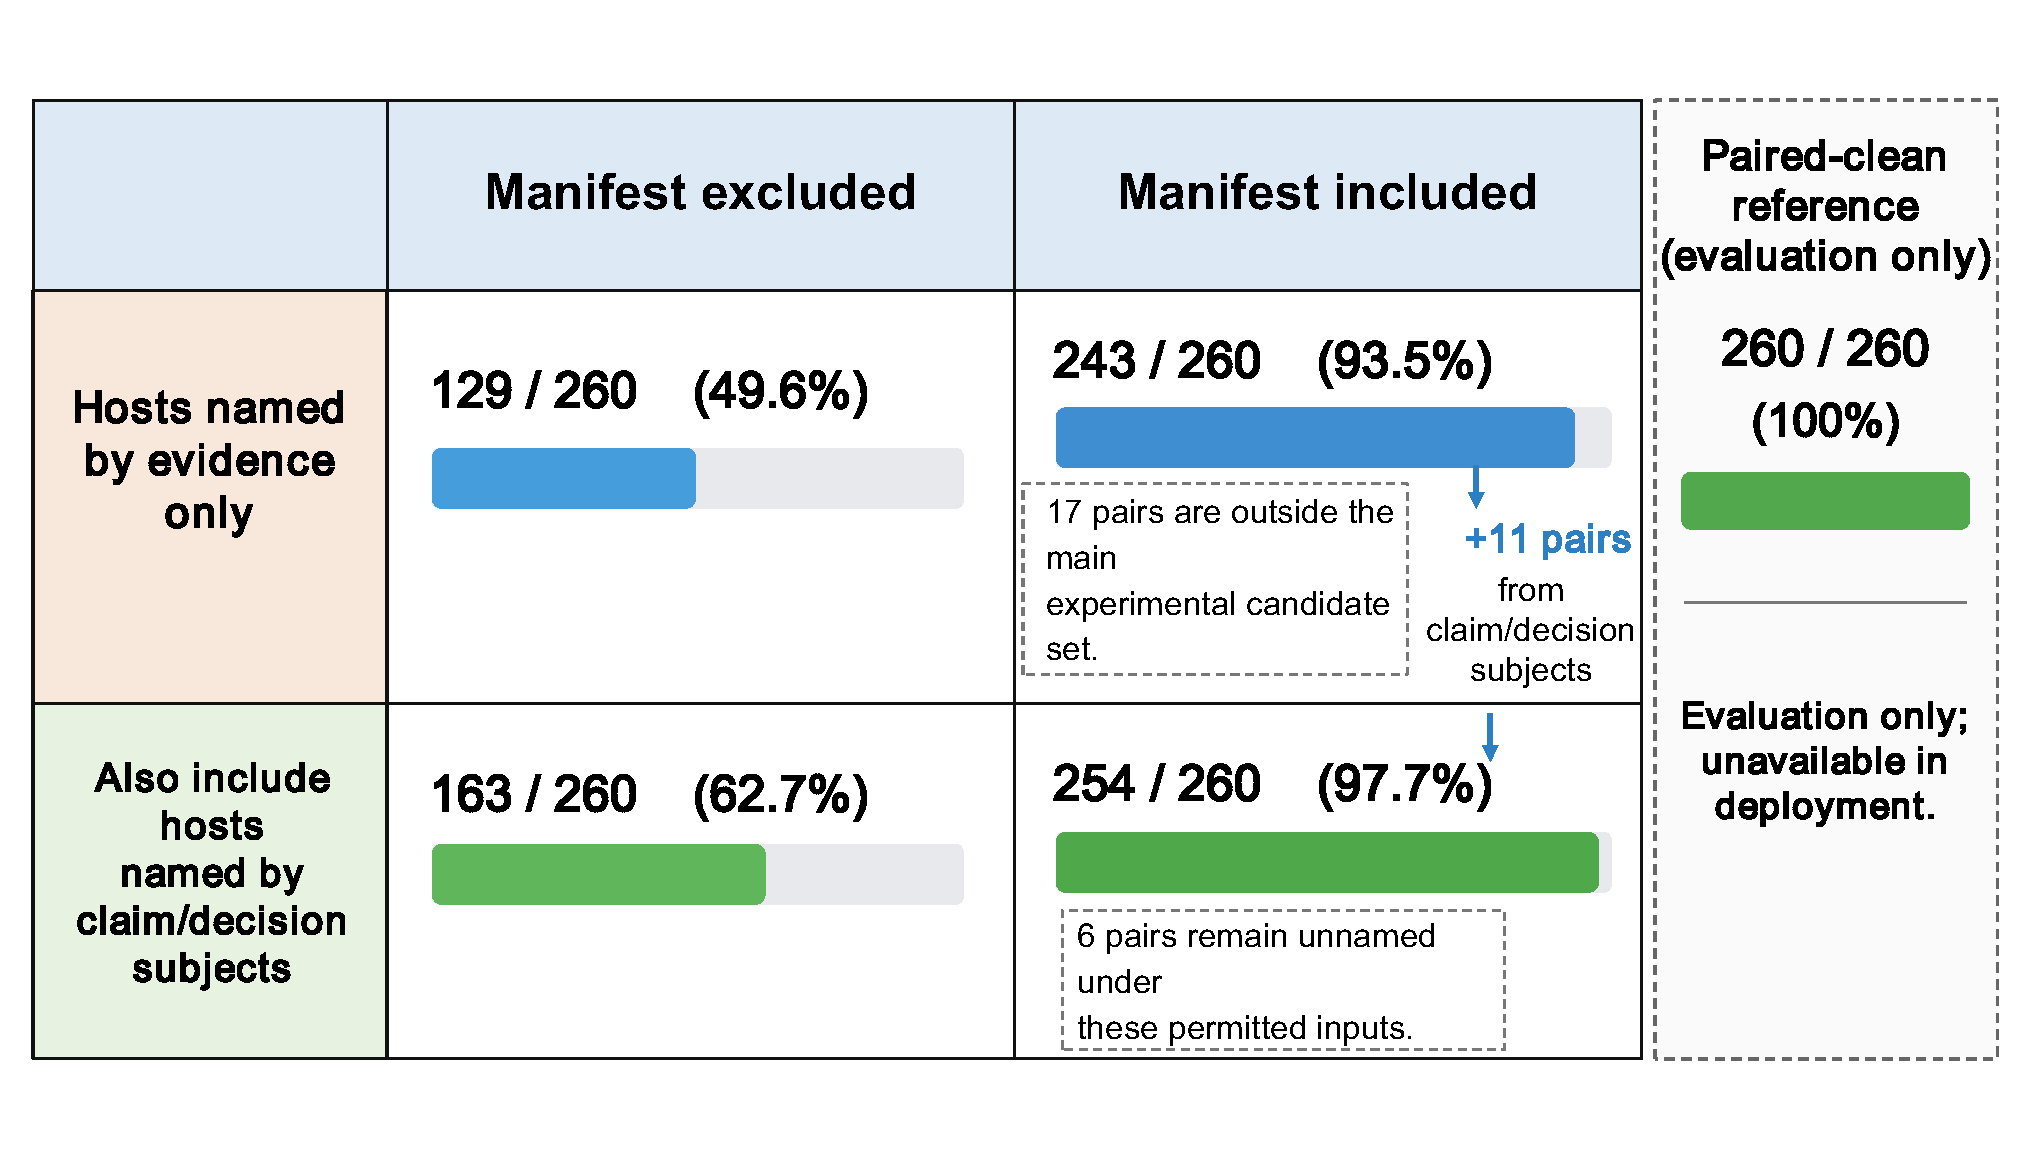
\includegraphics[width=\linewidth]{fig2}
\caption{Candidate visibility under alternative observation conditions. The paired-clean reference shows how many injected target identities were available before injection. The other conditions use records from the faulted run}
\label{fig:candidate-visibility}
\end{figure}

Across all 180 faulted runs, tie-aware Detect@1 was 0.735 for Combined (95\% CI \([0.686, 0.783]\)) and 0.456 for IF (95\% CI \([0.361, 0.556]\)). At rank three, the point estimates were 0.808 for Combined and 0.828 for IF. Across the 18,903 candidate rows pooled from the 180 faulted and 20 clean runs, candidate-conditional ROC AUC was 0.914 for Combined and 0.989 for IF. The 17 injected run--host pairs outside the faulted candidate sets contributed no rows to this AUC calculation.

Table~\ref{tab:host-ranking-alerting} reports ranking and alert results for the four methods in the main planner comparison.

\begin{table}[htbp]
\centering
\caption{Host ranking and alerting at the reported operating points}
\label{tab:host-ranking-alerting}
\small
\setlength{\tabcolsep}{2pt}
\renewcommand{\arraystretch}{1.1}
\begin{tabular*}{\linewidth}{@{\extracolsep{\fill}}lccccc@{}}
\toprule
Localizer &
Detect@1 &
\shortstack{Org-macro\\target-host\\alert recall} &
\shortstack{Alerted\\target-host\\pairs} &
\shortstack{Mean alerted\\hosts per\\faulted run} &
\shortstack{Org-macro\\clean-run\\alert rate} \\
\midrule
Combined    & 0.735 & 0.8194 & 221/260 & 11.57 & 0.1055 \\
IF          & 0.456 & 0.9417 & 243/260 &  9.18 & 0.1046 \\
Robust-\(z\) & 0.434 & 0.9361 & 242/260 & 10.79 & 0.1059 \\
Contract B  & 0.201 & 0.8250 & 222/260 & 20.55 & 0.1949 \\
\bottomrule
\end{tabular*}
\end{table}

Detect@1 averages the per-run top-1 hit probability over all 180 faulted runs. A tie for the highest score can give a run fractional credit (Section~\ref{sec:ranking-metrics}). Alerted target pairs are micro counts over 260 run--host pairs. Target-host recall and the clean-run alert rate are organization-macro averages. Alert volume is the mean number of alerted hosts per faulted run. IF exceeded Combined in organization-macro target-host recall by 12.22 percentage points (95\% bootstrap CI \([7.78, 16.67]\)). Combined used \(t=0.5\). IF and Robust-\(z\) used leave-one-organization-out calibration to the clean-run alert-rate target derived from Combined. Appendix~\ref{app:a-2} gives the LOF results.

In a post hoc comparison paired by organization, the mean Detect@1 difference across the nine variants was 0.280 in favor of Combined (95\% percentile bootstrap CI \([0.170, 0.391]\), 10,000 organization resamples, seed 42). IF had the higher Detect@1 for certificate omissions (0.800 versus 0.379) and registration omissions (0.850 versus 0.429). Combined had the higher rate for the other seven variants.

At the main operating points, IF flagged 22 more target pairs than Combined: 11 in \texttt{F4@certificate}, 10 in \texttt{F4@registration}, and one in \texttt{F4@active\_observation}. IF exceeded Combined in mean run-level alert recall by \(2/9\) in 11 organizations. The other nine showed no difference, giving an organization-macro difference of \((11/20)\times(2/9)\), or 12.22 percentage points. Section~\ref{sec:candidate-contract-sensitivity} compares paired clean and faulted alert status under the post hoc calibration.

\subsection{RQ3: Retrospective Common-Planner Analysis}
\label{sec:rq3-results}

Table~\ref{tab:common-planner} compares plan sufficiency and mean weighted specification cost across the four localizers.

\begin{table}[htbp]
\centering
\caption{Offline plan sufficiency (OPS) and mean weighted specification cost per run}
\label{tab:common-planner}
\small
\setlength{\tabcolsep}{4pt}
\renewcommand{\arraystretch}{1.1}
\begin{tabular*}{\linewidth}{@{\extracolsep{\fill}}lcrcr@{}}
\toprule
& \multicolumn{2}{c}{Selective}
& \multicolumn{2}{c}{Fixed-four} \\
\cmidrule(lr){2-3}\cmidrule(l){4-5}
Localizer & \shortstack{OPS, units\\covered (\%)} & Mean cost
          & \shortstack{OPS, units\\covered (\%)} & Mean cost \\
\midrule
Combined     & 119/180 (66.1\%) & 36.92 & 145/180 (80.6\%) &  69.43 \\
IF           & 142/180 (78.9\%) & 47.20 & 168/180 (93.3\%) &  55.07 \\
Robust-\(z\) & 141/180 (78.3\%) & 50.53 & 167/180 (92.8\%) &  64.77 \\
Contract B   & 120/180 (66.7\%) & 90.78 & 146/180 (81.1\%) & 123.30 \\
\bottomrule
\end{tabular*}
\end{table}

We summed the Table~\ref{tab:action-costs} weights of the distinct host--family actions in each plan and averaged the totals over all 180 runs, including runs with empty plans. With Combined alerts held fixed, fixed-four planning covered all required actions in 26 more runs than selective planning. The paired selective-minus-fixed difference in OPS was \(-0.144\) (95\% CI \([-0.200, -0.089]\)). The corresponding difference in mean weighted cost was \(-32.52\) (95\% CI \([-46.84, -20.05]\)). Certificate and registration omissions accounted for 19 of the 26 additional sufficient plans.

With fixed-four planning, IF alerts yielded sufficient plans in 168 of 180 runs and Combined alerts in 145. The paired IF-minus-Combined difference in OPS was \(+0.1278\) (95\% CI \([+0.0778, +0.1778]\)). Across all 180 runs, mean weighted specification cost was 55.07 with IF and 69.43 with Combined. The estimated difference was \(-14.37\) (95\% CI \([-46.03, +13.83]\)).

Table~\ref{tab:coverability-audit} separates required-action instances from run-level candidate coverability.

\begin{table}[htbp]
\centering
\caption{Required-action instance funnel and unit-level coverability audit}
\label{tab:coverability-audit}
\small
\setlength{\tabcolsep}{3pt}
\renewcommand{\arraystretch}{1.1}

\begin{tabularx}{\linewidth}{@{}l*{5}{>{\centering\arraybackslash}X}@{}}
\toprule
\multicolumn{6}{@{}l}{\textit{(a) Required host--family instances}} \\
\addlinespace[2pt]
Localizer & Required instances & Candidate-visible & On alerted hosts
          & Covered by selective plan & Covered by fixed-four plan \\
\midrule
Combined & 427 & 404 & 380 & 352 & 380 \\
IF       & 427 & 404 & 404 & 376 & 404 \\
\bottomrule
\end{tabularx}

\medskip

\begin{tabularx}{\linewidth}{@{}>{\raggedright\arraybackslash}Xrrr@{}}
\toprule
\multicolumn{4}{@{}l}{\textit{(b) Candidate coverability and IF fixed-four plan sufficiency (runs)}} \\
\addlinespace[2pt]
Candidate-coverability status & Sufficient & Insufficient & Total \\
\midrule
All required hosts admitted (\(U_i=1\))       & 168 &  0 & 168 \\
At least one required host absent (\(U_i=0\)) &   0 & 12 &  12 \\
\midrule
Total                                        & 168 & 12 & 180 \\
\bottomrule
\end{tabularx}
\end{table}

Of the 427 required host--family instances in Table~\ref{tab:coverability-audit}(a), 23 involved hosts outside the candidate set. A further 24 involved hosts that Combined did not flag. IF flagged hosts accounting for all 404 candidate-visible instances. Selective family choice left another 28 instances uncovered for each detector. Thus, the 75 instances not covered by the Combined selective plans comprise 23 candidate-invisible instances, 24 instances on hosts it did not alert, and 28 instances omitted by family selection.

Across the 260 injected run--host pairs, 243 targets entered the main candidate set. At least one injected host entered the set in 171 of 180 runs (Section~\ref{sec:rq2-results}). Panel~(b) asks whether every host with a required action entered the set. This occurred in 168 of 180 runs, establishing the observed upper bound on fixed-four plan sufficiency under this candidate rule. IF reached that bound.

\subsection{New-Location Sensitivity Analysis}\label{sec:new-location-sensitivity}

Table~\ref{tab:new-location-flow} summarizes the sample flow. Of 187 technically valid new locations, 186 had affected leaf-repairable outputs. These locations varied placement within the same frozen system.

\begin{table}[htbp]
\centering
\caption{New-location sample flow}
\label{tab:new-location-flow}
\small
\setlength{\tabcolsep}{3pt}
\renewcommand{\arraystretch}{1.12}
\begin{tabularx}{\linewidth}{@{}l*{4}{>{\centering\arraybackslash}X}@{}}
\toprule
Stratum & Sampled & \shortstack{Technically\\valid} & \shortstack{Consequence-\\eligible units} & \shortstack{Organizations\\with eligible\\units} \\
\midrule
DNS-only & 43 & 43 & 42 & 15 \\
DNS multi-family & 54 & 54 & 54 & 18 \\
Active observation & 90 & 90 & 90 & 18 \\
\midrule
Total & 187 & 187 & 186 & 18 distinct \\
\bottomrule
\end{tabularx}
\end{table}

The strata overlap in organization membership and together cover 18 distinct organizations. One technically valid DNS-only location had no affected leaf-repairable output.

All 43 DNS-only targets lacked a claim supplying an IP address for a manifest entry. At the 42 locations with affected leaf-repairable outputs, none of the targets appeared in \(E_i \cup R_i\), so all three localizers had Detect@1 of zero. Each location required one DNS action for its injected host. None of the saved plans covered that action.

Figure~\ref{fig:new-location} shows DNS-only target admission and Detect@1 by stratum.

\begin{figure}[htbp]
\centering
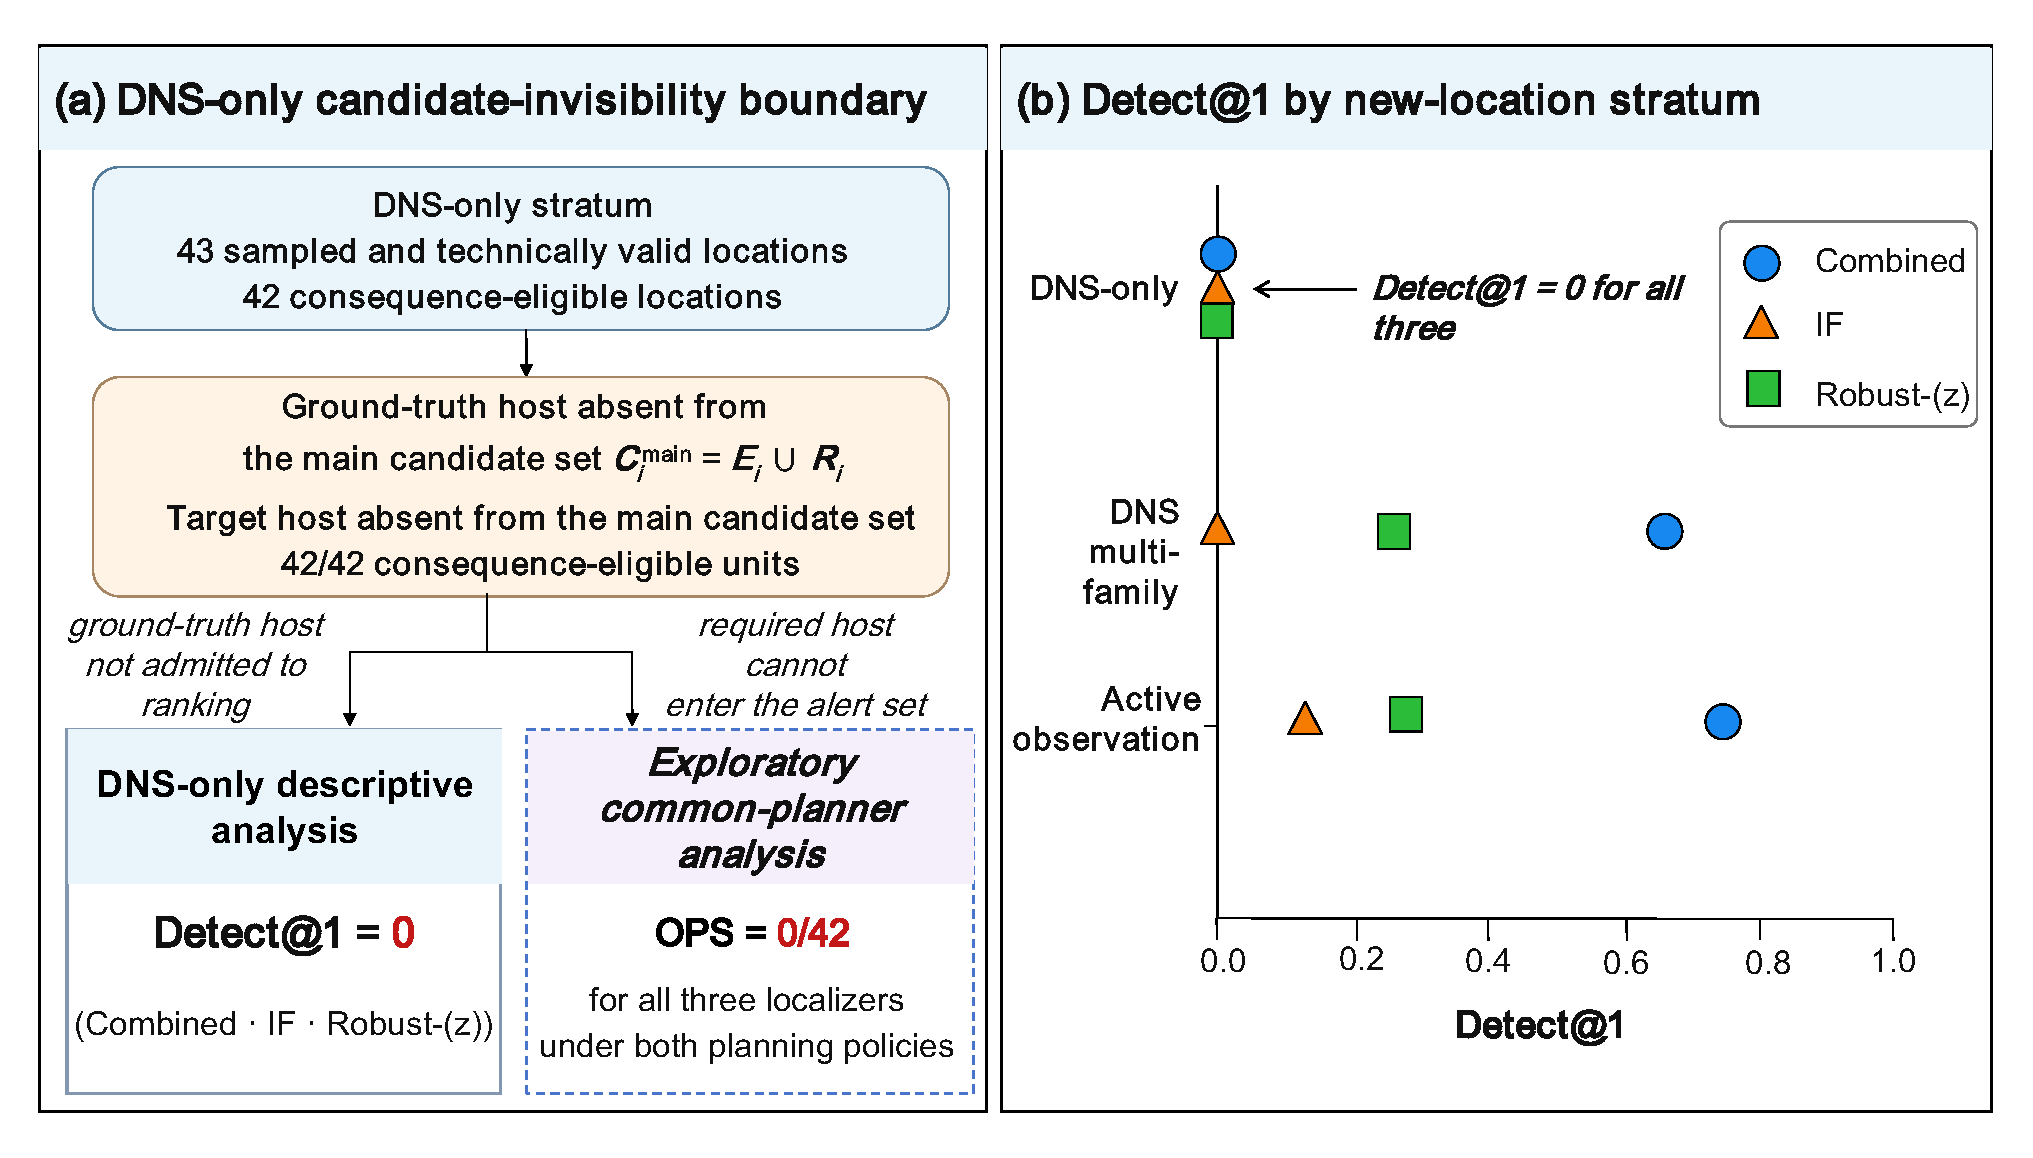
\includegraphics[width=\linewidth]{fig3}
\caption{New-location sensitivity and the DNS-only candidate-invisibility boundary. Panel (a) summarizes DNS-only target admission. Panel (b) shows Detect@1 by stratum; all three localizers have Detect@1 \(=0\) in the DNS-only stratum}
\label{fig:new-location}
\end{figure}

All four planned contrasts use 18 paired organizations and satisfy the reporting conditions defined in Section~\ref{sec:statistical-analysis}. Table~\ref{tab:planned-contrasts} reports estimates and adjusted intervals. Appendix~\ref{app:b} reports a post hoc check excluding the five locations previously targeted by other main-grid variants.

\begin{sidewaystable}[p]
\centering
\caption{Planned new-location contrasts and directional criteria}
\label{tab:planned-contrasts}
\small
\setlength{\tabcolsep}{3pt}
\renewcommand{\arraystretch}{1.12}
\begin{tabularx}{\linewidth}{@{}>{\raggedright\arraybackslash}Xcccccc@{}}
\toprule
Contrast & \shortstack{Paired\\organizations} & \shortstack{Consequence-\\eligible units} & \shortstack{Planned\\direction} & \shortstack{Estimate\\(Combined \(-\) IF)} & \shortstack{Two-sided 98.75\%\\Bonferroni-adjusted\\percentile bootstrap CI} & \shortstack{Directional\\criterion} \\
\midrule
P1: DNS multi-family Detect@1 & 18 & 54 & \(>0\) & \(+0.681\) & \([+0.500, +0.861]\) & CI entirely above 0 \\
P2: Active-observation Detect@1 & 18 & 90 & \(>0\) & \(+0.633\) & \([+0.422, +0.811]\) & CI entirely above 0 \\
P3: DNS multi-family archived \(C/C^{*}\) & 18 & 54 & \(<0\) & \(-14.43\) & \([-24.06, -3.62]\) & CI entirely below 0 \\
P4: Active-observation archived \(C/C^{*}\) & 18 & 90 & \(<0\) & \(-5.30\) & \([-8.28, -1.85]\) & CI entirely below 0 \\
\bottomrule
\end{tabularx}
\end{sidewaystable}

P1 and P2 estimate differences in Detect@1 proportions. P3 and P4 estimate differences in the dimensionless paired-clean scope-cost ratio \(C/C^{*}\) (Appendix~\ref{app:c}). Table~\ref{tab:planned-contrasts} reports the adjusted intervals used for all four planned contrasts. Appendix~\ref{app:b} reports their ordinary 95\% intervals, and Table~\ref{tab:app-c1} gives the absolute ratios for P3 and P4.

\subsection{Post Hoc Implementation and Operating-Point Sensitivities}\label{sec:operating-point-sensitivity}

We set manifest-only feature vectors to zero in clean and faulted runs and recalibrated the statistical baselines' thresholds. Aggregate target-alert counts and OPS were unchanged for IF and Robust-\(z\). For LOF, the alerted target-pair count and the number of sufficient plans under each policy increased by one (Appendix~\ref{app:a-1}).

The post hoc Combined threshold sweep used six sets of 180 saved run outcomes (Appendix~\ref{app:d-1}). Raising \(t\) from 0.5 to 0.7 left organization-macro target-host alert recall at 0.8194 and selective and fixed-four OPS at 119/180 and 145/180, respectively. Mean alerted hosts per run fell from 11.57 to 9.40. Mean weighted plan cost fell from 36.92 to 30.40 for selective planning (17.7\%) and from 69.43 to 56.40 for fixed-four planning (18.8\%).

At \(t=0.9\), fixed-four plans based on Combined alerts covered all required actions in 143/180 runs at a mean cost of 17.53 (Table~\ref{tab:app-d1}). Selective plans covered 119 runs with Combined alerts at \(t=0.5\) and 142 runs with IF alerts, at mean costs of 36.92 and 47.20, respectively (Table~\ref{tab:common-planner}). Combined fixed-four planning at \(t=0.9\) thus yielded one more sufficient run than IF selective planning. The thresholds and family-selection policies differed, and this post hoc comparison used no common clean-run calibration target. Appendix~\ref{app:d-2} reprices the saved plans using equal action weights.

\subsection{Exploratory Common-Planner Analysis at New Locations}\label{sec:new-location-planning}

In the DNS multi-family stratum, the tie-aware Detect@1 hit rate was 0.681 for Combined and 0.000 for IF. Both detectors flagged all 54 targets in the faulted runs. In the corresponding clean runs, Combined had flagged zero of these targets and IF had flagged seven. With either detector, both planning policies covered every required action in all 54 faulted runs.

Appendix~\ref{app:b} reports exploratory planning results for 42 DNS-only, 54 DNS multi-family, and 90 active-observation locations with eligible consequences. All policies had OPS of 0/42 in the DNS-only stratum. In each of the other two strata, both policies yielded the same OPS count for a given localizer, and selective plans had lower mean specification costs.

\subsection{Post Hoc Candidate-Contract and Common-Budget Sensitivity}\label{sec:candidate-contract-sensitivity}

For each clean and faulted bundle, we constructed both the main candidate set \(E \cup R\) and the expanded set \(C^{\mathrm{surv}} \cup R\). Under both rules, Combined looked up each admitted hostname in the same bundle-specific score map defined by its peer, validator, and manifest signals. It assigned zero to any hostname absent from the map. For each candidate set, we refitted IF on its feature matrix and recomputed Robust-\(z\) scores against its within-run peers. Under the expanded rule, the four-family assignment for manifest-only hosts in Section~\ref{sec:fault-input-planner} also applied to alerted hosts admitted through claims alone. In both cases the alerted host lacked surviving evidence.

For each detector and candidate rule, we calibrated a separate cutoff for each held-out organization using clean runs from the other 19. We ordered candidates lexicographically by (anomaly score, hostname hash) and flagged those whose pair was at or above the cutoff. Appendix~\ref{app:a-3} gives the hash construction. We considered the observed calibration pairs and a cutoff above all scores, selecting the cutoff with an organization-macro clean-run alert rate closest to 0.1055. If two rates were equally close, we chose the lower rate.

This procedure applies to the post hoc alert comparisons in Tables~\ref{tab:candidate-contract} and~\ref{tab:paired-alert-membership}. Table~\ref{tab:common-planner} uses the original operating points in Section~\ref{sec:stat-baselines}. Table~\ref{tab:candidate-contract} uses the nearest attainable calibration rate and the hostname tie-break described above. Detect@1 retains the tie-aware ranking definition in Section~\ref{sec:ranking-metrics}. Although both rules used the same calibration target, the held-out organization-macro clean-run alert rates varied by detector. Under either rule, they rounded to 0.1055 for Combined, 0.1070 for IF, and 0.1069 for Robust-\(z\).

Table~\ref{tab:candidate-contract} reports candidate-contract sensitivity under the common clean-run alert-rate target.

\begin{table}[htbp]
\centering
\caption{Post hoc candidate-contract sensitivity under a common clean-run alert-rate target. Each detector and candidate rule uses a recalibrated cutoff}
\label{tab:candidate-contract}
\small
\setlength{\tabcolsep}{3pt}
\renewcommand{\arraystretch}{1.12}
\begin{tabularx}{\linewidth}{@{}>{\raggedright\arraybackslash}Xrrr@{}}
\toprule
& \multicolumn{3}{c}{Main \(\to\) broad candidate rule} \\
\cmidrule(l){2-4}
Metric & Combined & IF & Robust-\(z\) \\
\midrule
Candidate coverage (of 260) & \(243 \to 254\) & \(243 \to 254\) & \(243 \to 254\) \\
Detect@1 & \(0.7355 \to 0.7355\) & \(0.4556 \to 0.4611\) & \(0.4338 \to 0.4366\) \\
Org-macro target-host alert recall & \(0.8194 \to 0.8194\) & \(0.9417 \to 0.9833\) & \(0.9417 \to 0.9833\) \\
Selective OPS (of 180) & \(119 \to 119\) & \(142 \to 151\) & \(142 \to 151\) \\
Fixed-four OPS (of 180) & \(145 \to 145\) & \(168 \to 177\) & \(168 \to 177\) \\
Fixed-four mean cost & \(69.43 \to 69.43\) & \(55.43 \to 55.63\) & \(65.87 \to 66.23\) \\
\bottomrule
\end{tabularx}
\end{table}

Candidate coverage counts target run--host pairs. Detect@1 and alert recall follow Section~\ref{sec:ranking-metrics}. OPS counts sufficient plans across all 180 faulted runs, and cost is the mean weighted plan cost per run. For both IF and Robust-\(z\), the paired difference in fixed-four OPS between the expanded and main rules was \(+0.0500\) (95\% CI \([0.0111, 0.0944]\)).

The expanded rule admitted 11 additional target pairs across nine DNS-omission runs. Four of the nine runs used single-host injections and five used two-host injections. Combined assigned its default score of zero to all 11 targets and flagged none. IF and Robust-\(z\) flagged all 11. For both statistical detectors, fixed-four plans became sufficient in exactly those nine runs, raising the total from 168 to 177 of 180. Every previously sufficient fixed-four plan remained sufficient. This comparison varies candidate admission, within-run scoring, and threshold calibration together.

Table~\ref{tab:paired-alert-membership} reports paired alert status under the main candidate rule. For each organization and detector, we applied the same cutoff to the clean and faulted runs. All 60 recalculated cutoffs matched the archived values and reproduced the 540 saved faulted-run alert sets.

\begin{table}[htbp]
\centering
\caption{Paired clean--faulted target alert membership for the main candidate rule under the post hoc common calibration budget}
\label{tab:paired-alert-membership}
\small
\setlength{\tabcolsep}{3pt}
\renewcommand{\arraystretch}{1.12}
\begin{tabularx}{\linewidth}{@{}>{\raggedright\arraybackslash}Xrrr@{}}
\toprule
Target alert status & Combined & IF & Robust-\(z\) \\
\midrule
\multicolumn{4}{@{}l}{\textit{Admitted to the faulted candidate set}} \\
Newly alerted & 199 & 152 & 143 \\
Alerted in both & 22 & 91 & 100 \\
Clean alert only & 0 & 0 & 0 \\
Alerted in neither & 22 & 0 & 0 \\
\addlinespace
\multicolumn{4}{@{}l}{\textit{Absent from the faulted candidate set}} \\
Alerted in clean & 6 & 0 & 3 \\
No clean alert & 11 & 17 & 14 \\
\midrule
Total & 260 & 260 & 260 \\
\bottomrule
\end{tabularx}
\end{table}

The first four data rows summarize alert status for the 243 target pairs admitted to the faulted candidate set. The next two data rows summarize clean-run alert status for the 17 target pairs absent from that set. A newly alerted host had no alert in the clean run and an alert in the faulted run.

\section{Discussion}\label{sec:discussion}

\subsection{Candidate Visibility and Identity Persistence}
\label{sec:identity-persistence}

Beyond the targets named in surviving evidence, the same-run manifest identified 91 additional F10 target pairs and 23 F4 pairs. Whether the manifest preserved an identity depended on whether the host had an asset entry with an IP address. None of the 42 consequence-eligible DNS-only targets had such an entry.

Retaining claim subjects can make a host available for inspection even when its name has no score in the original Combined map. The expanded rule assigned such hosts a default score of zero. An identity ledger would likewise need a policy for scoring newly admitted hosts.

\subsection{Ranking, Alert Coverage, and Plan Coverage}
\label{sec:ranking-alert-plan-coverage}

Across the nine variants, Combined had the higher tie-aware top-1 hit rate, while IF flagged more target pairs at the main operating points. The ordering depended on the omission: IF ranked targets first more often for certificate and registration omissions. The paired comparison under the post hoc common calibration target distinguishes new alerts from persistent ones (Table~\ref{tab:paired-alert-membership}). Combined newly flagged 199 target pairs and IF newly flagged 152. Of the pairs flagged in faulted runs, 91 had already been flagged by IF in the paired clean run, compared with 22 for Combined. Ranking guides the choice of which host to inspect first. Paired alert status shows whether that host's alert was new for the run.

Of the 427 required host--family instances, 23 involved hosts outside the main candidate set. A further 24 involved hosts that Combined did not flag, and selective family choice missed 28 more. Fixed-four plans covered all required families on alerted hosts at a higher mean weighted plan cost. Changing the Combined threshold changed the number of alerts and the cost of the resulting plans (Section~\ref{sec:operating-point-sensitivity}). A deployment study could evaluate thresholds, candidate rules, and family selection together under a declared clean-run alert budget.

\subsection{Host and Evidence-Family Uncertainty}
\label{sec:host-family-uncertainty}

Selective planning can omit certificate or registration actions when it selects other families and does not invoke the all-family fallback. Certificate and registration omissions accounted for 19 of the 26 additional runs covered by fixed-four plans with Combined alerts in the main grid. At new DNS multi-family and active-observation locations, the two policies had identical OPS counts within each detector. Executing a reacquisition plan would also require provider-specific operations for the abstract \texttt{active\_observation} action in Section~\ref{sec:action-contracts}.

\subsection{Implications for Software Engineering Practice}
\label{sec:practice-implications}

A run-scoped, append-only ledger could retain discovered hostnames and their source-stage identifiers before evidence collection. A replication could compare this ledger with \(E \cup R\) on both target coverage and the admission of stale names or aliases.

A replication in telemetry processing, incident analysis, or build systems could track which identifiers survive collection and aggregation before measuring how accurately a detector ranks the remaining candidates.

Alert thresholds also affect the scope of the resulting plans. For a given alert set, fixed-four planning sometimes covered requirements missed by selective planning. Its broader action scope increased the mean specification cost. A deployment study could set a clean-run alert budget in advance, evaluate candidate rules on held-out organizations or systems, and measure the resources consumed and evidence recovered when the planned actions are executed.

\subsection{Role of the LLM and Scope of Applicability}
\label{sec:llm-role-scope}

LLMs contributed to normalization, attribution, conflict resolution, and reporting in the replayed pipeline. The localizers ranked hosts using the structured records that survived those stages. The study evaluated how omissions at two specified boundaries affected diagnosis. The retained records do not establish how individual upstream model decisions contributed to each omission's downstream effects. Evaluating closed-loop recovery would require executing the planned actions and observing what evidence they recovered.

\section{Threats to Validity}\label{sec:threats-to-validity}

\subsection{Construct Validity}\label{sec:construct-validity}

\textbf{Plan and cost constructs.} OPS measures whether a saved plan includes the required actions. Provider-specific reacquisition may require different requests, and the relative family weights do not measure execution time or resource use (Section~\ref{sec:offline-planning}).

\textbf{Candidate contract.} The broader surviving-record analysis includes post hoc recalibration and downstream outcomes (Section~\ref{sec:candidate-contract-sensitivity}), but remains conditional on this corpus, candidate implementation, and calibration budget.

\textbf{Reference labels and diagnostic signals.} We reproduced the archived \(F_1\) values using the retained labels, although the original input checksums were unavailable. Some merged port labels contained values absent from the retained source-specific fields (Appendix~\ref{app:d-3}). Incomplete labels limit conclusions about real-world asset coverage. The separate prediction-set comparison in Section~\ref{sec:rq1-results} establishes which measured outputs remained identical. Unavailable runtime telemetry also limits what can be inferred about omission-identifying signals beyond the persisted records.

\subsection{Internal Validity}\label{sec:internal-validity}

The original target-selection rules favored evidence-rich hosts. Such targets may be easier to retain or reconstruct from surviving records, so the main results may understate the difficulty of locating hosts with sparse evidence. The additional injections varied placement within the same corpus and revealed this limitation in the DNS-only stratum.

Using the protocol-specified zero vectors for the 23 affected manifest-only rows changed some scores. Aggregate alert counts and OPS were unchanged for IF and Robust-\(z\), while the LOF sufficient-plan count increased by one under each policy (Appendix~\ref{app:a-1}). Main-grid planning comparisons were retrospective and new-location planning was exploratory.

In one \texttt{F10-local} run, the evaluator identified two required host--family actions on hosts other than the injected target. With plans held fixed, restricting the evaluator to injected-host actions increased the number of sufficient plans by one under each policy for Combined (selective, 119 to 120 of 180; fixed-four, 145 to 146) and Contract B (120 to 121 and 146 to 147, respectively). The counts for IF and Robust-\(z\) were unchanged.

For F4, we replayed the full pipeline with the omission enabled during decision-stage normalization. Table~\ref{tab:paired-alert-membership} describes the paired clean and faulted alert states. In the new-location study, all 18 organization-level clean preflight replays matched their frozen baselines on the recorded checks. After the engineering pilot, the versioned protocol allowed a statistics-only summary when the report-summary cache missed. This fallback occurred after decision construction in 131 of the 187 formal new-location runs. Other LLM cache misses still terminated the run. In the pilot, the saved structured outputs matched with and without the fallback. Its effect on report items in each of the 131 formal runs was not independently verified. The main grid lacked a contemporaneous no-injection replay for each faulted run, which limits attribution of individual alert changes to the injection.

\subsection{External Validity}\label{sec:external-validity}

The evidence comes from one external reconnaissance pipeline, one frozen corpus, and 20 purposively selected organizations. New-location tests varied fault placement within the same system and included eligible units from 18 organizations. The proposed parallels with telemetry processing, build lineage, and automated operations remain hypotheses. Testing their applicability requires replications that vary both the system and the candidate-admission rule \citep{shull2008}.

\subsection{Conclusion Validity}\label{sec:conclusion-validity}

Candidate visibility and micro alert recall use 260 run--host pairs. Main-grid Detect@\(k\) and OPS use 180 faulted runs. At new locations, we report OPS within strata drawn from 186 consequence-eligible units. Candidate-conditional AUC uses pooled candidate rows. Organization-macro estimates first average within each organization and then across organizations. Section~\ref{sec:statistical-analysis} specifies the four new-location contrasts in the Bonferroni family. Intervals for comparisons outside that family are descriptive.

\section{Conclusion}\label{sec:conclusion}

Across 20 purposively selected organizations, adding the same-run manifest raised target coverage from 129 to 243 of 260 injected run--host pairs. Combined ranked a target first more often than IF. The candidate sets contained every host required for offline plan sufficiency in 168 of 180 runs. Fixed-four plans based on IF alerts covered all required actions in all 168, compared with 145 runs for Combined. At the additional DNS-only locations, all 42 consequence-eligible targets fell outside the candidate set, and none of the plans covered the required DNS action.

These results support measuring candidate admission, ranking, alerting, and required-action coverage separately. Under the expanded rule and its corresponding scoring and calibration procedures, plans based on IF and Robust-\(z\) alerts were sufficient in more runs, while the number of sufficient plans based on Combined alerts was unchanged. Future replications could compare candidate-admission rules across pipelines and test whether executing the planned actions restores the required evidence.

\backmatter

\section*{Statements and Declarations}

\subsection*{Research Ethics and Dual-Use Considerations}

The localizers flagged candidate hosts, and the planner specified evidence to reacquire for each alerted host. We evaluated these plans offline and executed none of the planned actions against production hosts. This statement applies to the evaluated plans. The records of the original data collection are incomplete (Section~\ref{sec:main-sample}).

The study involved no human participants or animals. Historical network records may contain personal or other sensitive information. We report aggregate results and one pseudonymous host example. Access to the underlying host records is restricted.

\subsection*{Data Availability}

The analysis code, evaluation scripts, and aggregate figures and tables reported in this study will be available from the project repository at \url{https://github.com/chenxuan0248-a11y/DYMAM-analysis-code} upon publication. Host-level prediction records, per-run result JSON, and original reconnaissance bundles are not included. Some underlying raw reconnaissance data may be requested from the corresponding author, subject to applicable data-use terms, privacy safeguards, and review; access cannot be guaranteed.

\subsection*{Funding}

No funding was received for conducting this study.

\subsection*{Competing Interests}

The authors declare no competing interests.

\subsection*{Author Contributions}

Xuan Chen, Kai Yi, and Haodong Wang contributed to the study design, conducted the experiments, analyzed the data, and wrote the manuscript. Xiangmin Ji supervised the study. All authors reviewed and approved the final manuscript and accept responsibility for its contents.

\subsection*{Generative AI Use}

During manuscript preparation in October--November 2026, the authors used OpenAI ChatGPT to help organize and edit the manuscript, draft portions of the analysis scripts, and perform exploratory consistency checks. The authors reviewed and ran the scripts and checked the results against the archived records.

This assistance was separate from the LLM components used in the experimental pipeline. ChatGPT did not generate experimental labels or ground truth. The authors take responsibility for the study design, analysis methods, references, figures and tables, interpretation of the results, and final manuscript.

\begin{appendices}

\renewcommand*{\theHtable}{appendix.\Alph{section}.\arabic{table}}

\section{Implementation Sensitivity and Supplementary LOF Results}\label{app:a}

\setcounter{table}{0}

\subsection{Manifest-Only Forced-Zero Sensitivity}\label{app:a-1}

The executed implementation retained claim/decision features for 23 manifest-only rows, contrary to the protocol's zero-vector rule. Anomaly-detection methods differ in their assumptions about normal behavior \citep{chandola2009}. In the forced-zero sensitivity, both clean and faulted feature vectors were transformed, clean-run thresholds recalibrated, and scores, alerts, and plans recomputed. Table~\ref{tab:app-a1} summarizes the resulting implementation sensitivity.

\begin{table}[htbp]
\centering
\caption{Manifest-only forced-zero implementation sensitivity}
\label{tab:app-a1}
\small
\setlength{\tabcolsep}{3pt}
\renewcommand{\arraystretch}{1.1}
\begin{tabular*}{\linewidth}{@{\extracolsep{\fill}}llccccc@{}}
\toprule
Method & \shortstack{Feature\\condition} & \shortstack{Alerted\\target pairs} & \shortstack{Selective\\OPS} & \shortstack{Fixed-four\\OPS} & \shortstack{Selective\\mean cost} & \shortstack{Fixed-four\\mean cost} \\
\midrule
IF & Implemented & 243/260 & 142/180 & 168/180 & 47.20 & 55.07 \\
IF & Forced-zero & 243/260 & 142/180 & 168/180 & 47.22 & 54.97 \\
\addlinespace
Robust-\(z\) & Implemented & 242/260 & 141/180 & 167/180 & 50.53 & 64.77 \\
Robust-\(z\) & Forced-zero & 242/260 & 141/180 & 167/180 & 50.37 & 64.60 \\
\addlinespace
LOF & Implemented & 119/260 & 62/180 & 82/180 & 55.03 & 61.03 \\
LOF & Forced-zero & 120/260 & 63/180 & 83/180 & 54.96 & 60.97 \\
\bottomrule
\end{tabular*}
\end{table}

Under the forced-zero condition, detector scores changed in 22/180 faulted runs for IF, 19/180 for Robust-\(z\), and 22/180 for LOF. For IF and Robust-\(z\), aggregate target-host alert counts and OPS were unchanged, although score vectors and mean specification costs changed. For LOF, the alerted target-pair count increased by one, as did the number of sufficient plans under each policy.

\subsection{Supplementary LOF Results}\label{app:a-2}

LOF uses the manifest-aware statistical feature representation and leave-one-organization-out, clean-only threshold calibration. The planning results below use the same frozen main grid and fault-input common planner as the other statistical baselines. Table~\ref{tab:app-a2} reports its supplementary ranking, alert, and planning results.

\begin{table}[htbp]
\centering
\caption{LOF results under the executed implementation}
\label{tab:app-a2}
\small
\setlength{\tabcolsep}{3pt}
\renewcommand{\arraystretch}{1.1}
\begin{tabularx}{\linewidth}{@{}Xr@{}}
\toprule
Measure & LOF \\
\midrule
Detect@1 & 0.328 \\
Clean-run alert rate, org-macro & 0.1082 \\
Target-host alert recall, org-macro & 0.4639 \\
Alerted target-host pairs, micro & 119/260 \\
Selective OPS & 62/180 \\
Fixed-four OPS & 82/180 \\
Selective mean cost & 55.03 \\
Fixed-four mean cost & 61.03 \\
\bottomrule
\end{tabularx}
\end{table}

The clean-run alert rate and target-host alert recall are organization-macro averages, while \(119/260\) counts alerted target run--host pairs. Table~\ref{tab:app-a1} gives the corresponding forced-zero result.

\subsection{Sampling seeds and calibration tie-breaking}\label{app:a-3}

Each draw used NumPy's PCG64 generator initialized with the pair \texttt{[20261008, child\_seed]}. To derive the child seed, we encoded \verb!organization|stratum|role! in UTF-8, computed its SHA-256 digest, and read the first eight bytes as an unsigned big-endian integer. The stratum strings were \texttt{dns\_only}, \texttt{dns\_multi}, and \texttt{ao}. The role was either \texttt{pilot} or \texttt{formal}.

For the post hoc calibration in Section~\ref{sec:candidate-contract-sensitivity}, we concatenated the prefix \verb!alert-budget-v1|! and the stored hostname, encoded the result in UTF-8, and computed its SHA-256 digest. For the secondary key, we interpreted the first 16 hexadecimal digits as an unsigned integer and divided it by \(2^{64}\).

\section{Additional Analyses at the Sampled Locations}\label{app:b}

\setcounter{table}{0}

The common-planner analysis at new locations was specified after the new-location localization results were known and is therefore exploratory.

The ordinary two-sided 95\% bootstrap intervals for the four planned contrasts are P1 [0.5278, 0.8194], P2 [0.4778, 0.7778], P3 [\ensuremath{-}22.2407, \ensuremath{-}6.2963], and P4 [\ensuremath{-}7.7000, \ensuremath{-}2.7849]. Table~\ref{tab:planned-contrasts} reports the corresponding two-sided 98.75\% Bonferroni-adjusted intervals used for directional interpretation.

Sample flow and eligibility counts appear in Table~\ref{tab:new-location-flow}. Table~\ref{tab:app-b1} reports the exploratory planner outcomes. Detect@1, target-host alert recall, and cost are equal-weight organization means within each stratum; OPS is the fraction of consequence-eligible units covered.

\begin{sidewaystable}[p]
\centering
\caption{Exploratory common-planner results at new locations}
\label{tab:app-b1}
\small
\setlength{\tabcolsep}{3pt}
\renewcommand{\arraystretch}{1.1}
\begin{tabular*}{\linewidth}{@{\extracolsep{\fill}}llrrrrrr@{}}
\toprule
Stratum & Localizer & Detect@1 & \shortstack{Org-macro\\target-host\\alert recall} & \shortstack{Selective\\OPS} & \shortstack{Selective\\mean cost} & \shortstack{Fixed-four\\OPS} & \shortstack{Fixed-four\\mean cost} \\
\midrule
DNS-only & Combined & 0.000 & 0.000 & 0/42 & 32.47 & 0/42 & 64.40 \\
DNS-only & IF & 0.000 & 0.000 & 0/42 & 52.07 & 0/42 & 59.60 \\
DNS-only & Robust-\(z\) & 0.000 & 0.000 & 0/42 & 54.27 & 0/42 & 66.40 \\
\addlinespace
DNS multi-family & Combined & 0.681 & 1.000 & 54/54 & 30.28 & 54/54 & 64.00 \\
DNS multi-family & IF & 0.000 & 1.000 & 54/54 & 39.50 & 54/54 & 51.89 \\
DNS multi-family & Robust-\(z\) & 0.255 & 1.000 & 54/54 & 49.00 & 54/54 & 65.56 \\
\addlinespace
Active observation & Combined & 0.767 & 0.978 & 88/90 & 34.34 & 88/90 & 63.87 \\
Active observation & IF & 0.133 & 1.000 & 90/90 & 45.81 & 90/90 & 54.00 \\
Active observation & Robust-\(z\) & 0.261 & 0.889 & 80/90 & 52.81 & 80/90 & 64.87 \\
\bottomrule
\end{tabular*}
\end{sidewaystable}

In the DNS-only stratum, plans could incur costs by specifying actions for other hosts even though none covered the required DNS action for the target.

\textbf{Sensitivity to previously targeted hosts.} We repeated the four Table~\ref{tab:planned-contrasts} contrasts after excluding the five locations whose hosts had been targeted by a different main-grid variant. This post hoc check retained 53 DNS multi-family locations and 86 active-observation locations, with 18 organizations in each stratum. We used the same within-organization averaging and organization-level bootstrap as in Section~\ref{sec:statistical-analysis}. Table~\ref{tab:app-b2} reports these sensitivity estimates.

\begin{table}[htbp]
\centering
\caption{Paired contrasts after excluding hosts targeted by other main-grid variants}
\label{tab:app-b2}
\small
\setlength{\tabcolsep}{3pt}
\renewcommand{\arraystretch}{1.1}
\begin{tabularx}{\linewidth}{@{}>{\raggedright\arraybackslash}Xrc@{}}
\toprule
Contrast (Combined minus IF) & Estimate & \shortstack{Two-sided 98.75\%\\Bonferroni-adjusted\\percentile interval} \\
\midrule
P1 DNS multi-family, Detect@1 & +0.681 & [+0.500, +0.861] \\
P2 Active observation, Detect@1 & +0.664 & [+0.451, +0.847] \\
P3 DNS multi-family, \(C/C^{*}\) & \ensuremath{-}14.54 & [\ensuremath{-}24.25, \ensuremath{-}3.69] \\
P4 Active observation, \(C/C^{*}\) & \ensuremath{-}5.30 & [\ensuremath{-}8.30, \ensuremath{-}1.87] \\
\bottomrule
\end{tabularx}
\end{table}

\section{Paired-Clean Scope Evaluation for P3 and P4}\label{app:c}

\setcounter{table}{0}

P3 and P4 use an evaluation-only paired-clean scope analysis that is separate from the fault-input common planner used for the main RQ3 OPS and specification-cost results.

\subsection{Operational construction}\label{app:c-1}

For unit \(i\) and detector \(m\), let \(A_{m,i}\) be the host alerts generated from faulted-run inputs. The evaluator maps these fixed alerts to the paired clean graph.

\begin{enumerate}

\item \textbf{Detector-induced scope.} The Step-2 implementation selects repairable nodes in the paired-clean DAG whose \texttt{target} is in \(A_{m,i}\), normalizes their source family using \texttt{cost\_harm\_spec.yaml}, and deduplicates canonical invocations by \texttt{(target, source\_family)}. With \(\Psi_i(A_{m,i})\) denoting that set and \(w(f)\) its configured family cost,

\[
C_{m,i}=\sum_{(h,f)\in\Psi_i(A_{m,i})}w(f).
\]

\item \textbf{Paired-clean ILP oracle.} The retained P3/P4 evaluator entry calls \texttt{solve\_oracle(clean, faulted)} without supplying alternative coverage sets; in the inspected call path, this invokes the default single-required-set formulation. Let \(\mathcal{O}_i\) denote affected outputs and \(\mathcal{A}_i\) eligible repair invocations. For every \(o\), \(R_i(o)\subseteq\mathcal{A}_i\) contains its complete required invocation set. Binary variable \(x_a\) selects an invocation with cost \(c(a)\) and harm \(h(a)\):

\[
\begin{aligned}
\min_{x}\quad &
   \alpha\sum_{a\in\mathcal{A}_i} c(a)x_a
   + \beta\sum_{a\in\mathcal{A}_i} h(a)x_a \\
\text{subject to}\quad &
   x_a=1 && \forall o\in\mathcal{O}_i,\; \forall a\in R_i(o), \\
& \sum_{a\in\mathcal{A}_i} h(a)x_a \le H_{\max}, \\
& x_a=0 && \forall a\text{ classified irreversible}, \\
& x_a\in\{0,1\} && \forall a\in\mathcal{A}_i.
\end{aligned}
\]

The retained \texttt{ilp\_config.yaml} specifies \(\alpha=\beta=1\), \(H_{\max}=93\), full required-set coverage, and exclusion of irreversible actions. The archived consequence-eligible new-location evaluations report \texttt{Optimal} solver status and positive \(C_i^{*}\) for all 186 units.

\item \textbf{Reported reference-cost component.} Let \(\Omega_i^{*}=\{a:x_a^{*}=1\}\) be the invocation set selected by the constrained ILP. The quantity used as the P3/P4 denominator is

\[
C_i^{*}=\sum_{a\in\Omega_i^{*}}c(a),\qquad C_i^{*}>0,
\]

the cost component of the optimal feasible solution. We used the same family mapping and deduplication by \texttt{(target, source\_family)} for the oracle and detector-induced scopes.

\item \textbf{Aggregation.} We calculated \(q_{m,i}=C_{m,i}/C_i^{*}\) for each unit, averaged the ratios within each organization and stratum, and computed paired organization-level Combined-minus-IF differences. Confidence intervals follow the organization bootstrap and four-comparison Bonferroni scheme in Section~\ref{sec:statistical-analysis}.

\end{enumerate}

In the archived implementation, \texttt{p1b\_evaluate.py} aggregates the P3/P4 ratios, \texttt{step2\_baselines.py} selects the detector-induced scope, and \texttt{ilp\_oracle.py} implements the constrained oracle.

\subsection{Absolute ratios underlying P3 and P4}\label{app:c-2}

Table~\ref{tab:app-c1} reports the organization-macro \(C/C^{*}\) values underlying P3 and P4. This dimensionless ratio divides the detector-induced scope cost by the cost component of the constrained optimum on the paired-clean graph. Section~\ref{sec:action-contracts} prices the main-grid plan specifications separately. OPS records whether a plan covers all required actions.

\begin{table}[htbp]
\centering
\caption{Organization-macro \(C/C^{*}\) values underlying P3 and P4}
\label{tab:app-c1}
\small
\setlength{\tabcolsep}{3pt}
\renewcommand{\arraystretch}{1.1}
\begin{tabularx}{\linewidth}{@{}Xccrrr@{}}
\toprule
Stratum & \shortstack{Paired\\orgs.} & \shortstack{Eligible\\units} & \shortstack{Combined\\\(C/C^{*}\)} & \shortstack{IF\\\(C/C^{*}\)} & \shortstack{Combined\\\ensuremath{-} IF} \\
\midrule
DNS multi-family & 18 & 54 & 14.2778 & 28.7037 & \ensuremath{-}14.4259 \\
Active observation & 18 & 90 & 4.7370 & 10.0370 & \ensuremath{-}5.3000 \\
\bottomrule
\end{tabularx}
\end{table}

The values yield the rounded main-text contrasts of \ensuremath{-}14.43 for DNS multi-family and \ensuremath{-}5.30 for active observation. A lower ratio indicates lower scope cost under this paired-clean evaluator, but does not by itself establish higher plan sufficiency; coverage and OPS are evaluated separately.

\subsection{Provenance status}\label{app:c-3}

The archived solver returned an optimal feasible solution for all 186 eligible units under the single-required-set formulation. The archive records matching hashes for the entry script, protocol, sampling list, and Step-2 artifacts. The historical versions of some imported dependencies and configuration files could not be established.

\section{Sensitivity Analyses for Alert Thresholds, Cost Weights, and Port Labels}\label{app:d}

\setcounter{table}{0}

Using the saved snapshot, we varied the Combined alert threshold (D.1), repriced the saved plans with equal action weights (D.2), and examined the sensitivity of port F1 to source-specific reference fields (D.3).

\subsection{Combined Alert-Threshold Sensitivity}\label{app:d-1}

The threshold sweep changes only the Combined host-alert cutoff \(t\). The selective planner's family-prevalence cutoff remains fixed at 0.5.

We averaged clean-run alert rates across the 20 organizations and evaluated OPS across all 180 main-grid faulted runs. We averaged plan cost within organizations and then weighted organizations equally. Because each contributed nine runs, this also gives the mean across runs.

\begin{sidewaystable}[p]
\centering
\caption{Post hoc Combined alert and planning sensitivity across thresholds}
\label{tab:app-d1}
\small
\setlength{\tabcolsep}{3pt}
\renewcommand{\arraystretch}{1.1}
\begin{tabular*}{\linewidth}{@{\extracolsep{\fill}}crrrrrr@{}}
\toprule
t & \shortstack{Org-macro\\clean alert rate} & \shortstack{Org-macro\\target-host recall} & \shortstack{Alerted target\\pairs (micro)} & \shortstack{Mean alerted\\hosts/run} & \shortstack{Selective OPS\\(mean cost)} & \shortstack{Fixed-four OPS\\(mean cost)} \\
\midrule
0.3 & 0.1949 & 0.8250 & 222/260 & 20.17 & 120/180 (88.52) & 146/180 (121.03) \\
0.4 & 0.1613 & 0.8194 & 221/260 & 17.16 & 119/180 (70.45) & 145/180 (102.97) \\
0.5 & 0.1055 & 0.8194 & 221/260 & 11.57 & 119/180 (36.92) & 145/180 (69.43) \\
0.6 & 0.1055 & 0.8194 & 221/260 & 11.57 & 119/180 (36.92) & 145/180 (69.43) \\
0.7 & 0.0872 & 0.8194 & 221/260 & 9.40 & 119/180 (30.40) & 145/180 (56.40) \\
0.9 & 0.0195 & 0.8083 & 219/260 & 2.92 & 117/180 (10.97) & 143/180 (17.53) \\
\bottomrule
\end{tabular*}
\end{sidewaystable}

Table~\ref{tab:app-d1} uses 1,080 saved threshold--run outcomes (six thresholds \(\times\) 180 runs). Target recall is organization-macro, alerted target pairs are micro counts, and alert volume is the mean per faulted run. Parentheses in the final two columns give mean weighted specification cost.

The \(t=0.5\) row reproduces the main Combined results. At \(t=0.7\), recall and both OPS counts were unchanged, while alert volume and mean costs fell alongside the clean-run alert rate. This post hoc sweep varied only the Combined threshold; it does not identify an optimal threshold because no alert-cost utility function was specified in advance.

\subsection{Equal-Weight Cost Sensitivity}\label{app:d-2}

The main analysis assigns relative specification-cost weights of 1 to DNS, certificate, and registration actions and 3 to active-observation actions. To assess dependence on this weighting choice, we repriced the saved plans by assigning one unit to every distinct \((\mathrm{host},\mathrm{family})\) action. Table~\ref{tab:app-d2} gives the resulting action counts.

\begin{table}[htbp]
\centering
\caption{Equal-weight action counts for the saved main-grid plans}
\label{tab:app-d2}
\small
\setlength{\tabcolsep}{3pt}
\renewcommand{\arraystretch}{1.1}
\begin{tabularx}{\linewidth}{@{}Xcrcr@{}}
\toprule
Localizer & \shortstack{Selective\\OPS} & \shortstack{Selective mean\\host--family actions} & \shortstack{Fixed-four\\OPS} & \shortstack{Fixed-four mean\\host--family actions} \\
\midrule
Combined & 119/180 & 14.54 & 145/180 & 46.29 \\
IF & 142/180 & 29.61 & 168/180 & 36.71 \\
Robust-\(z\) & 141/180 & 29.71 & 167/180 & 43.18 \\
Contract B & 120/180 & 50.45 & 146/180 & 82.20 \\
\bottomrule
\end{tabularx}
\end{table}

With equal weights, the mean plan cost is the mean number of distinct \((\mathrm{host},\mathrm{family})\) actions specified per plan.

The repricing covered 1,440 saved plans across 180 faulted runs, four localizers, and two planning policies.

\subsection{Port-label sensitivity using retained source-specific fields}\label{app:d-3}

All 1,149 organization--subdomain reference rows contained a \texttt{ports} key, and 800 had a nonempty merged port list. In 318 rows, that list included values absent from the union of \texttt{ports\_shodan} and \texttt{ports\_censys}. We replaced each merged list with the union of the two source-specific lists and held predictions fixed. Missing source-specific lists contributed no ports to the union. All 318 discrepant rows had an empty \texttt{gt\_sources} field, leaving the provenance of the additional merged port values unresolved. The source-specific fields may also omit ports. Table~\ref{tab:app-d3} summarizes the resulting port-F1 sensitivity.

\begin{table}[htbp]
\centering
\caption{Port-\(F_1\) sensitivity to retained source-specific port fields}
\label{tab:app-d3}
\small
\setlength{\tabcolsep}{3pt}
\renewcommand{\arraystretch}{1.1}
\begin{tabular*}{\linewidth}{@{\extracolsep{\fill}}lcrrc@{}}
\toprule
Variant & Units & \shortstack{Clean mean\\port \(F_1\)} & \shortstack{Faulted mean\\port \(F_1\)} & \shortstack{Paired port\\\(F_1\) equal} \\
\midrule
\texttt{F4@dns} & 20 & 0.184621 & 0.184621 & 20/20 \\
\texttt{F4@certificate} & 20 & 0.184621 & 0.184621 & 20/20 \\
\texttt{F4@registration} & 20 & 0.184621 & 0.184621 & 20/20 \\
\texttt{F4-2host-dns} & 20 & 0.184621 & 0.184621 & 20/20 \\
\texttt{F4@active\_observation} & 20 & 0.184621 & 0.182493 & 9/20 \\
\texttt{F4-host} & 20 & 0.184621 & 0.180412 & 9/20 \\
\texttt{F10-local} & 20 & 0.184621 & 0.182493 & 9/20 \\
\texttt{F10-2host} & 20 & 0.184621 & 0.177979 & 8/20 \\
\texttt{F10-3host} & 20 & 0.184621 & 0.173066 & 8/20 \\
\bottomrule
\end{tabular*}
\end{table}

For the four F4 variants with identical paired port predictions, any common reference set necessarily yields identical clean and faulted port F1. Across the other five variants, the source-specific reference sets yielded equal paired port F1 in 8 or 9 of the 20 runs per variant (Table~\ref{tab:app-d3}).

\end{appendices}

\clearpage
\bibliography{sn-bibliography}
\end{document}
